\documentclass[a4paper, 11pt]{article}	
\usepackage[margin=1.75cm]{geometry} 
\usepackage{listings}
\usepackage[utf8]{inputenc}
\usepackage[russian]{babel}
\usepackage{setspace}
\usepackage{tikz}
\usepackage{pgfplots}
\usepackage{graphicx}
\usepackage{float}
\usepackage{xcolor}
\usepackage{fancyhdr}
\usepackage{colortbl}
\setlength{\parindent}{0pt}
\pgfplotsset{width=11cm,compat=1.3}
\setcounter{tocdepth}{3}

\pagestyle{fancy}
\fancyhf{}
\fancyhead[C]{\textit{Суперкомпьютеры и параллельная обработка данных}}
\fancyfoot[C]{\thepage}


\lstset{
    language=C, % Язык программирования
    basicstyle=\small\ttfamily, % Базовый стиль шрифта и размер
    numbers=left, % Нумерация строк слева (заменено на допустимое значение)
    numberstyle=\tiny\color{gray}, % Стиль нумерации строк
    stepnumber=1, % Шаг нумерации строк
    numbersep=5pt, % Расстояние между номером строки и кодом
    backgroundcolor=\color{gray!10}, % Фоновый цвет
    showspaces=false, % Показывать пробелы в коде?
    showstringspaces=false, % Показывать пробелы в строках?
    showtabs=false, % Показывать табуляцию?
    tabsize=4, % Размер табуляции
    captionpos=b, % Позиция заголовка
    breaklines=false, % Автоматический перенос строк
    breakatwhitespace=false, % Разрывать строки только по пробелам?
    escapeinside={\%*}{*)}, % Для вставки комментариев в коде
    keywordstyle=\color{blue}, % Стиль ключевых слов
    commentstyle=\color{green!40!black}, % Стиль комментариев
    stringstyle=\color{red}, % Стиль строк
    morekeywords={*, uint8_t, uint16_t, uint32_t, uint64_t, int8_t, int16_t, int32_t, int64_t, inline, restrict}, % Дополнительные ключевые слова
}


\begin{document}

\begin{titlepage}
    \begin{center}
        \vspace*{1cm}

        \Huge
        \textbf{Практикум по курсу} \\
        \LARGE
        <<Суперкомпьютеры и параллельная обработка данных>>

        \vspace{3cm}

        \Huge
        \textbf{Отчет о выполненном задании} \\
        \Large
        студента 321 учебной группы \\
        факультета ВМК МГУ

        \vspace{0.5cm}

        \LARGE
        Теслюка Никиты Сергеевича

        \vspace{3cm}

        \Large
        \textbf{Лектор:} доцент, к.ф.-м.н. Бахтин Владимир Александрович

        \vspace{5cm}

        \Large
        Вариант 43

        \vfill

        \Large
        Москва, 2024г. 

    \end{center}
\end{titlepage}
\tableofcontents
\newpage

\section*{Постановка задачи}
\addcontentsline{toc}{section}{Постановка задачи}

Цель работы — разработка параллельной программы для решения задачи численного моделирования давления в задаче на уравнение Пуассона с использованием метода Якоби. \\

В рамках работы необходимо:

\begin{enumerate}
    \item Реализовать параллельные программы с использованием OpenMP на языке программирования \texttt{C}:
    \begin{itemize}
        \item с директивой \texttt{for} для распределения витков циклов;
        \item с директивой \texttt{task} для механизма задач;
    \end{itemize}
    \item Реализовать параллельную программу с использованием MPI.
    \item Исследовать эффективность программ.
    \begin{itemize}
        \item Исследовать влияние различных опций оптимизации, которые поддерживаются компиляторами (\texttt{-O2}, \texttt{-O3}). 
    \end{itemize}
    \item Исследовать масштабируемость программ: построить графики зависимости времени от числа ядер и объёма данных для разных версий программы.
    \item Проанализировать причины ограниченной масштабируемости при максимальном числе ядер.
\end{enumerate}

\newpage

\section*{Описание последовательного алгоритма}
\addcontentsline{toc}{section}{Описание исходного алгоритма}

Программа реализует итерационную схему для решения задачи давления методом Якоби, используемого в решателе линейных уравнений для уравнения Пуассона давления в задаче о некомпрессируемом течении жидкости на языке \texttt{C}. Алгоритм работает на трехмерной сетке с разреженными коэффициентами.

\subsection*{Используемые функции}
\addcontentsline{toc}{subsection}{Используемые функции}

\begin{itemize}
    \item \texttt{main()} — инициализация матриц, запуск итераций метода Якоби и измерение производительности (время выполнения и операции с плавающей запятой).
    \item \texttt{initmt()} — инициализация матриц, задание начальных значений для элементов массива сетки и коэффициентов для вычисления давления и граничных условий.
    \item \texttt{jacobi(int nn)} — обновление значений давления и расчет сходимости на каждом шаге, вычисление ошибки (\texttt{gosa}), показателя сходимости.
    \item \texttt{second()} — измерение времени выполнения итераций. В будущем, при распараллеливании, будет использована функция \texttt{omp\_get\_wtime()} в случае использования OMP и \texttt{MPI\_Wtime()} в случае использования MPI.
\end{itemize}

\subsection*{Используемые переменные}
\addcontentsline{toc}{subsection}{Используемые переменные}

Программа использует следующие массивы:

\begin{itemize}
    \item \texttt{imax, jmax, kmax} — переменные для хранения размеров решаемой области (по осям x, y, z).
    \item \texttt{omega} — параметр релаксации для метода Якоби (находится в диапазоне от 0 до 1).
    \item \texttt{NN} — количество итераций для выполнения в цикле метода Якоби.
    \item \texttt{cpu0, cpu1} — переменные для измерения времени выполнения программы.
    \item \texttt{gosa} — переменная для хранения значения ошибки (остаточного) в процессе вычислений.
    \item \texttt{p[MIMAX][MJMAX][MKMAX]} — трехмерный массив для хранения давления в сетке.
    \item \texttt{a[MIMAX][MJMAX][MKMAX][4]} — массив коэффициентов для уравнения Пуассона (размерность 4 для каждого элемента).
    \item \texttt{b[MIMAX][MJMAX][MKMAX][3]} — массив коэффициентов для уравнения Пуассона (размерность 3 для каждого элемента).
    \item \texttt{c[MIMAX][MJMAX][MKMAX][3]} — массив коэффициентов для уравнения Пуассона (размерность 3 для каждого элемента).
    \item \texttt{wrk1[MIMAX][MJMAX][MKMAX]} — рабочий массив для хранения промежуточных значений (источник члена уравнения Пуассона).
    \item \texttt{wrk2[MIMAX][MJMAX][MKMAX]} — рабочий массив для хранения результатов промежуточных вычислений.
    \item \texttt{bnd[MIMAX][MJMAX][MKMAX]} — массив для граничных условий (значения 0 или 1, определяющие, является ли точка на границе или нет).
\end{itemize}

\vspace{0.3cm}

\begin{center}
    \begin{tabular}{l|l l l l}
            & \texttt{SMALL} & \texttt{MIDDLE} & \texttt{LARGE} & \texttt{EXTLARGE} \\
            \hline
            \texttt{MIMAX} & $65$   & $129$  & $257$  & $513$ \\
            \texttt{MJMAX} & $33$   & $65$   & $129$  & $257$ \\
            \texttt{MKMAX} & $33$   & $65$   & $129$  & $257$ \\
    \end{tabular} \\
    \vspace{0.3cm}
    \small \it
    Таблица 0. Размеры входных данных.
\end{center}
\newpage


\section*{OpenMP}
\addcontentsline{toc}{section}{OpenMP}
\subsection*{Параллелизация при помощи директивы \texttt{for}}
\addcontentsline{toc}{subsection}{Параллелизация при помощи директивы \texttt{for}}

\subsubsection*{Внесенные изменения}
\addcontentsline{toc}{subsubsection}{Внесенные изменения}

Для преобразования последовательной программы в параллельную с использованием директивы for OpenMP были внесены следующие изменения:

\begin{itemize}
    \item Для параллелизации циклов использована директива \texttt{\#pragma omp parallel for}, которая делегирует выполнение итераций цикла параллельным потокам.
    \item Директива \texttt{\#pragma omp parallel} используется для создания параллельной области, позволяя нескольким потокам работать одновременно.
    \item Директива \texttt{collapse(3)} объединяет три вложенных цикла, увеличивая эффективность распределения работы между потоками.
    \item Для переменной \texttt{gosa} применена директива \texttt{reduction(+:gosa)}, которая создает локальные копии переменной для каждого потока. По завершении параллельных вычислений локальные значения складываются в глобальную переменную.
    \item Директива \texttt{schedule(static)} задает равномерное распределение работы между потоками до начала выполнения.
    \item \texttt{private(i, j, k)} гарантирует, что переменные индексов цикла \texttt{i}, \texttt{j}, \texttt{k} будут локальными для каждого потока, исключая конфликты между потоками.
\end{itemize}
\newpage

\subsubsection*{Код программы}
\addcontentsline{toc}{subsubsection}{Код программы}
\begin{lstlisting}
#include <stdio.h>
#include <omp.h>

#define MIDDLE

#ifdef SMALL
#define MIMAX 65
#define MJMAX 33
#define MKMAX 33
#endif

#ifdef MIDDLE
#define MIMAX 129
#define MJMAX 65
#define MKMAX 65
#endif

#ifdef LARGE
#define MIMAX 257
#define MJMAX 129
#define MKMAX 129
#endif

#ifdef EXTLARGE
#define MIMAX 513
#define MJMAX 257
#define MKMAX 257
#endif

#define NN 200

static float p[MIMAX][MJMAX][MKMAX];
static float a[MIMAX][MJMAX][MKMAX][4], 
             b[MIMAX][MJMAX][MKMAX][3], c[MIMAX][MJMAX][MKMAX][3];
static float bnd[MIMAX][MJMAX][MKMAX];
static float wrk1[MIMAX][MJMAX][MKMAX], wrk2[MIMAX][MJMAX][MKMAX];

static int imax, jmax, kmax;
static float omega;

void
initmt()
{
    int i, j, k;
    
#pragma omp parallel for collapse(3) private(i, j, k)
    for (i = 0; i < imax; ++i) {
        for (j = 0; j < jmax; ++j) {
            for (k = 0; k < kmax; ++k) {
                a[i][j][k][0] = 0.0;
                a[i][j][k][1] = 0.0;
                a[i][j][k][2] = 0.0;
                a[i][j][k][3] = 0.0;
                b[i][j][k][0] = 0.0;
                b[i][j][k][1] = 0.0;
                b[i][j][k][2] = 0.0;
                c[i][j][k][0] = 0.0;
                c[i][j][k][1] = 0.0;
                c[i][j][k][2] = 0.0;
                p[i][j][k] = 0.0;
                wrk1[i][j][k] = 0.0;
                bnd[i][j][k] = 0.0;
            }
        }
    }
#pragma omp parallel for collapse(3) private(i, j, k)
    for (i = 0; i < imax; ++i) {
        for (j = 0; j < jmax; ++j) {
            for (k = 0; k < kmax; ++k) {
                a[i][j][k][0] = 1.0;
                a[i][j][k][1] = 1.0;
                a[i][j][k][2] = 1.0;
                a[i][j][k][3] = 1.0 / 6.0;
                c[i][j][k][0] = 1.0;
                c[i][j][k][1] = 1.0;
                c[i][j][k][2] = 1.0;
                p[i][j][k] = (float) (k * k) /
                             (float) ((kmax - 1) * (kmax - 1));
                wrk1[i][j][k] = 0.0;
                bnd[i][j][k] = 1.0;
            }
        }
    }
}

float
jacobi(int nn)
{
    int i, j, k, n;
    float gosa, s0, ss;

    for (n = 0; n < nn; ++n) {
        gosa = 0.0;

#pragma omp parallel shared(a, b, c, p, wrk1, wrk2, bnd, gosa) 
private(i, j, k, s0, ss)
        {
#pragma omp for schedule(static) collapse(3) reduction(+ : gosa)
            for (i = 1; i < imax - 1; ++i) {
                for (j = 1; j < jmax - 1; ++j) {
                    for (k = 1; k < kmax - 1; ++k) {
                        s0 = a[i][j][k][0] * p[i + 1][j][k] +
                             a[i][j][k][1] * p[i][j + 1][k] +
                             a[i][j][k][2] * p[i][j][k + 1] +
                             b[i][j][k][0] * (p[i + 1][j + 1][k] -
                                              p[i + 1][j - 1][k] -
                                              p[i - 1][j + 1][k] +
                                              p[i - 1][j - 1][k]) +
                             b[i][j][k][1] * (p[i][j + 1][k + 1] -
                                              p[i][j - 1][k + 1] -
                                              p[i][j + 1][k - 1] +
                                              p[i][j - 1][k - 1]) +
                             b[i][j][k][2] * (p[i + 1][j][k + 1] -
                                              p[i - 1][j][k + 1] -
                                              p[i + 1][j][k - 1] +
                                              p[i - 1][j][k - 1]) +
                             c[i][j][k][0] * p[i - 1][j][k] +
                             c[i][j][k][1] * p[i][j - 1][k] +
                             c[i][j][k][2] * p[i][j][k - 1] +
                             wrk1[i][j][k];


                        ss = (s0 * a[i][j][k][3] - p[i][j][k]) *
                              bnd[i][j][k];

                        gosa = gosa + ss * ss;

                        wrk2[i][j][k] = p[i][j][k] + omega * ss;
                    }
                }
            }

#pragma omp for schedule(static) collapse(3)
            for (i = 1; i < imax - 1; ++i) {
                for (j = 1; j < jmax - 1; ++j) {
                    for (k = 1; k < kmax - 1; ++k) {
                        p[i][j][k] = wrk2[i][j][k];
                    }
                }
            }
        }
    }
    return gosa;
}


int
main()
{
    int i, j, k;
    float gosa;
    double cpu0, cpu1, nflop, xmflops2, score;
    omega = 0.8;
    imax = MIMAX - 1;
    jmax = MJMAX - 1;
    kmax = MKMAX - 1;

    initmt();

    printf("mimax = %d mjmax = %d mkmax = %d\n", MIMAX, MJMAX, MKMAX);
    printf("imax = %d jmax = %d kmax =%d\n", imax, jmax, kmax);

    cpu0 = omp_get_wtime();

    gosa = jacobi(NN);

    cpu1 = omp_get_wtime();

    nflop = (kmax - 2) * (jmax - 2) * (imax - 2) * 34;

    if (cpu1 != 0.0) {
        xmflops2 = nflop / cpu1 * 1.0e-6 * (float) NN;
    }

    score = xmflops2 / 32.27;

    printf("cpu : %f sec.\n", cpu1 - cpu0);
    printf("Loop executed for %d times\n", NN);
    printf("Gosa : %e \n", gosa);
    printf("MFLOPS measured : %f\n", xmflops2);
    printf("Score based on MMX Pentium 200MHz : %f\n", score);

    return (0);
}
\end{lstlisting}
\newpage


\subsubsection*{Тестирование программы на Polus}
\addcontentsline{toc}{subsubsection}{Тестирование программы на Polus}

\begin{center}
    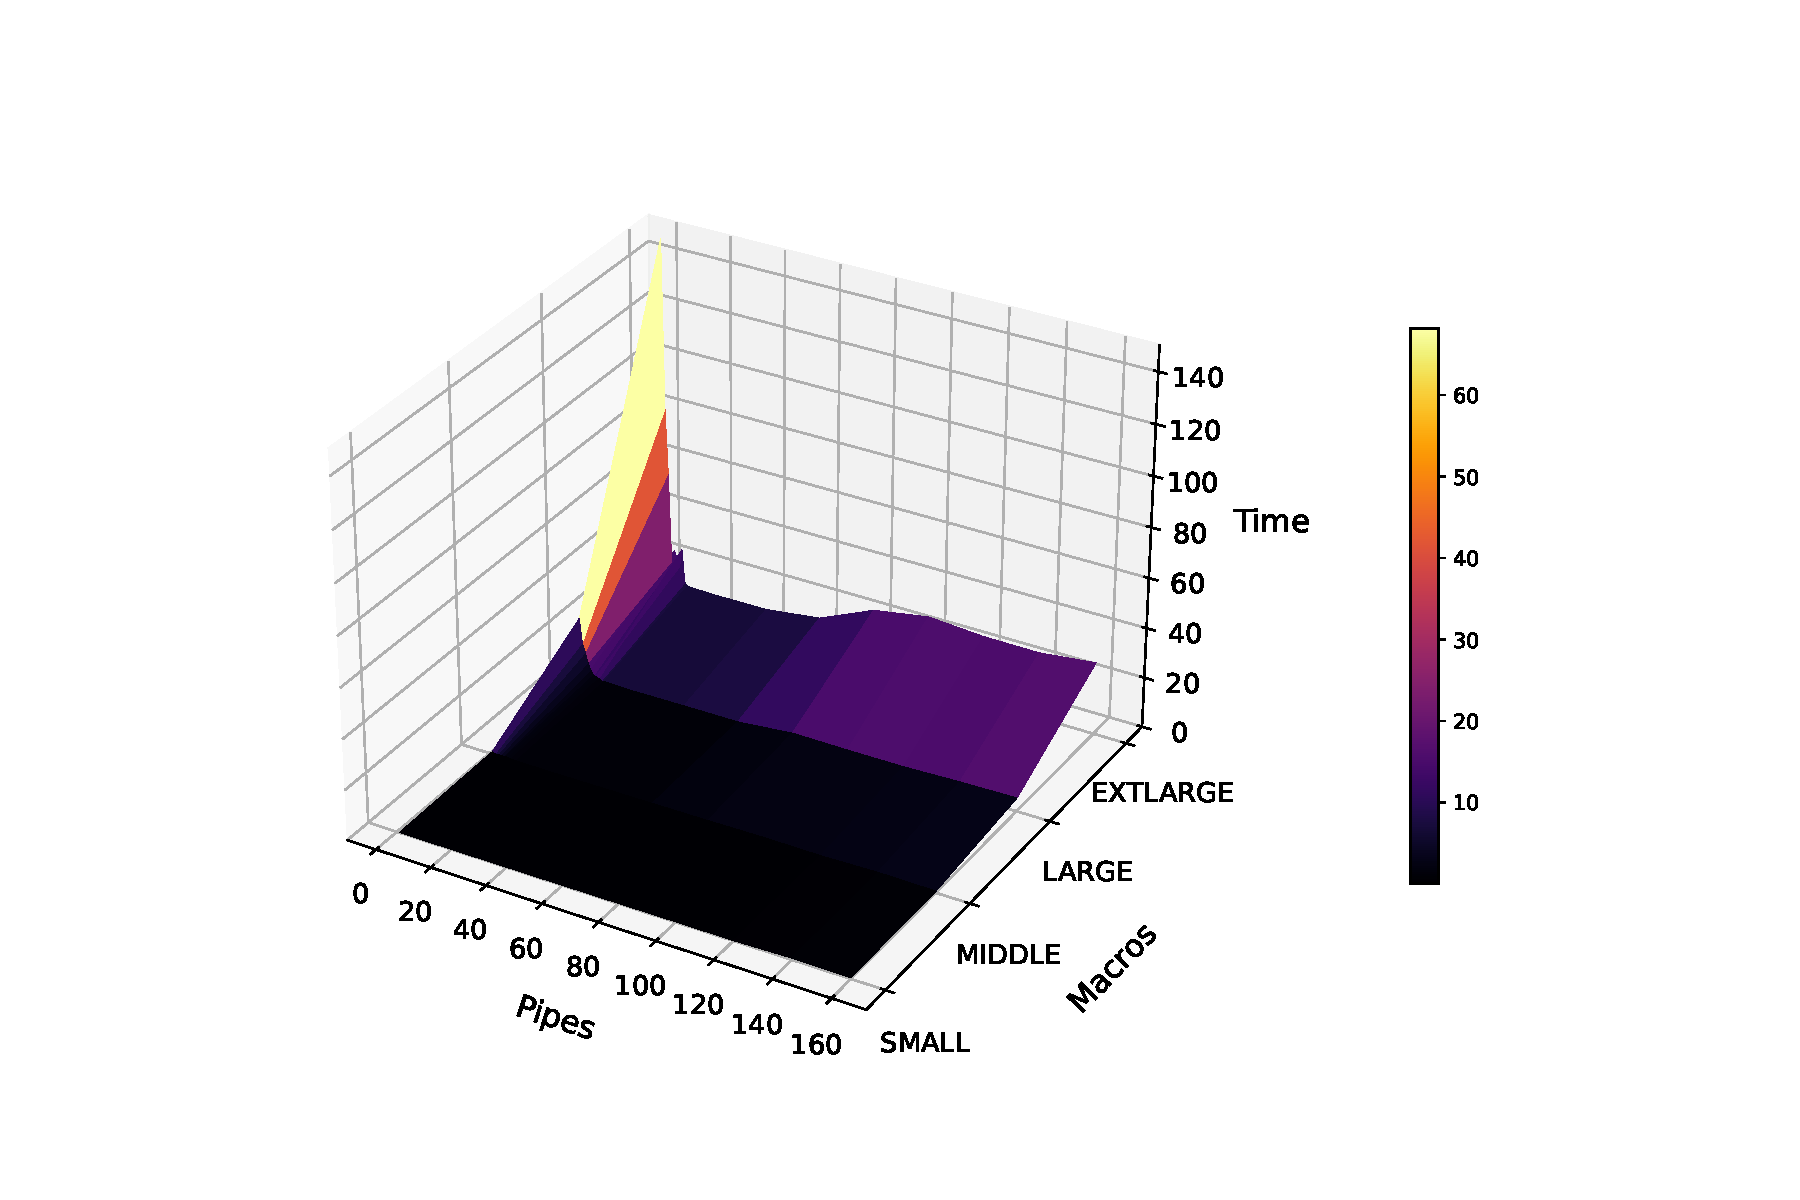
\includegraphics[width=0.8\textwidth]{../graph/for.pdf} \\
    \small \it
    График 1.1
\end{center}

\begin{center}
    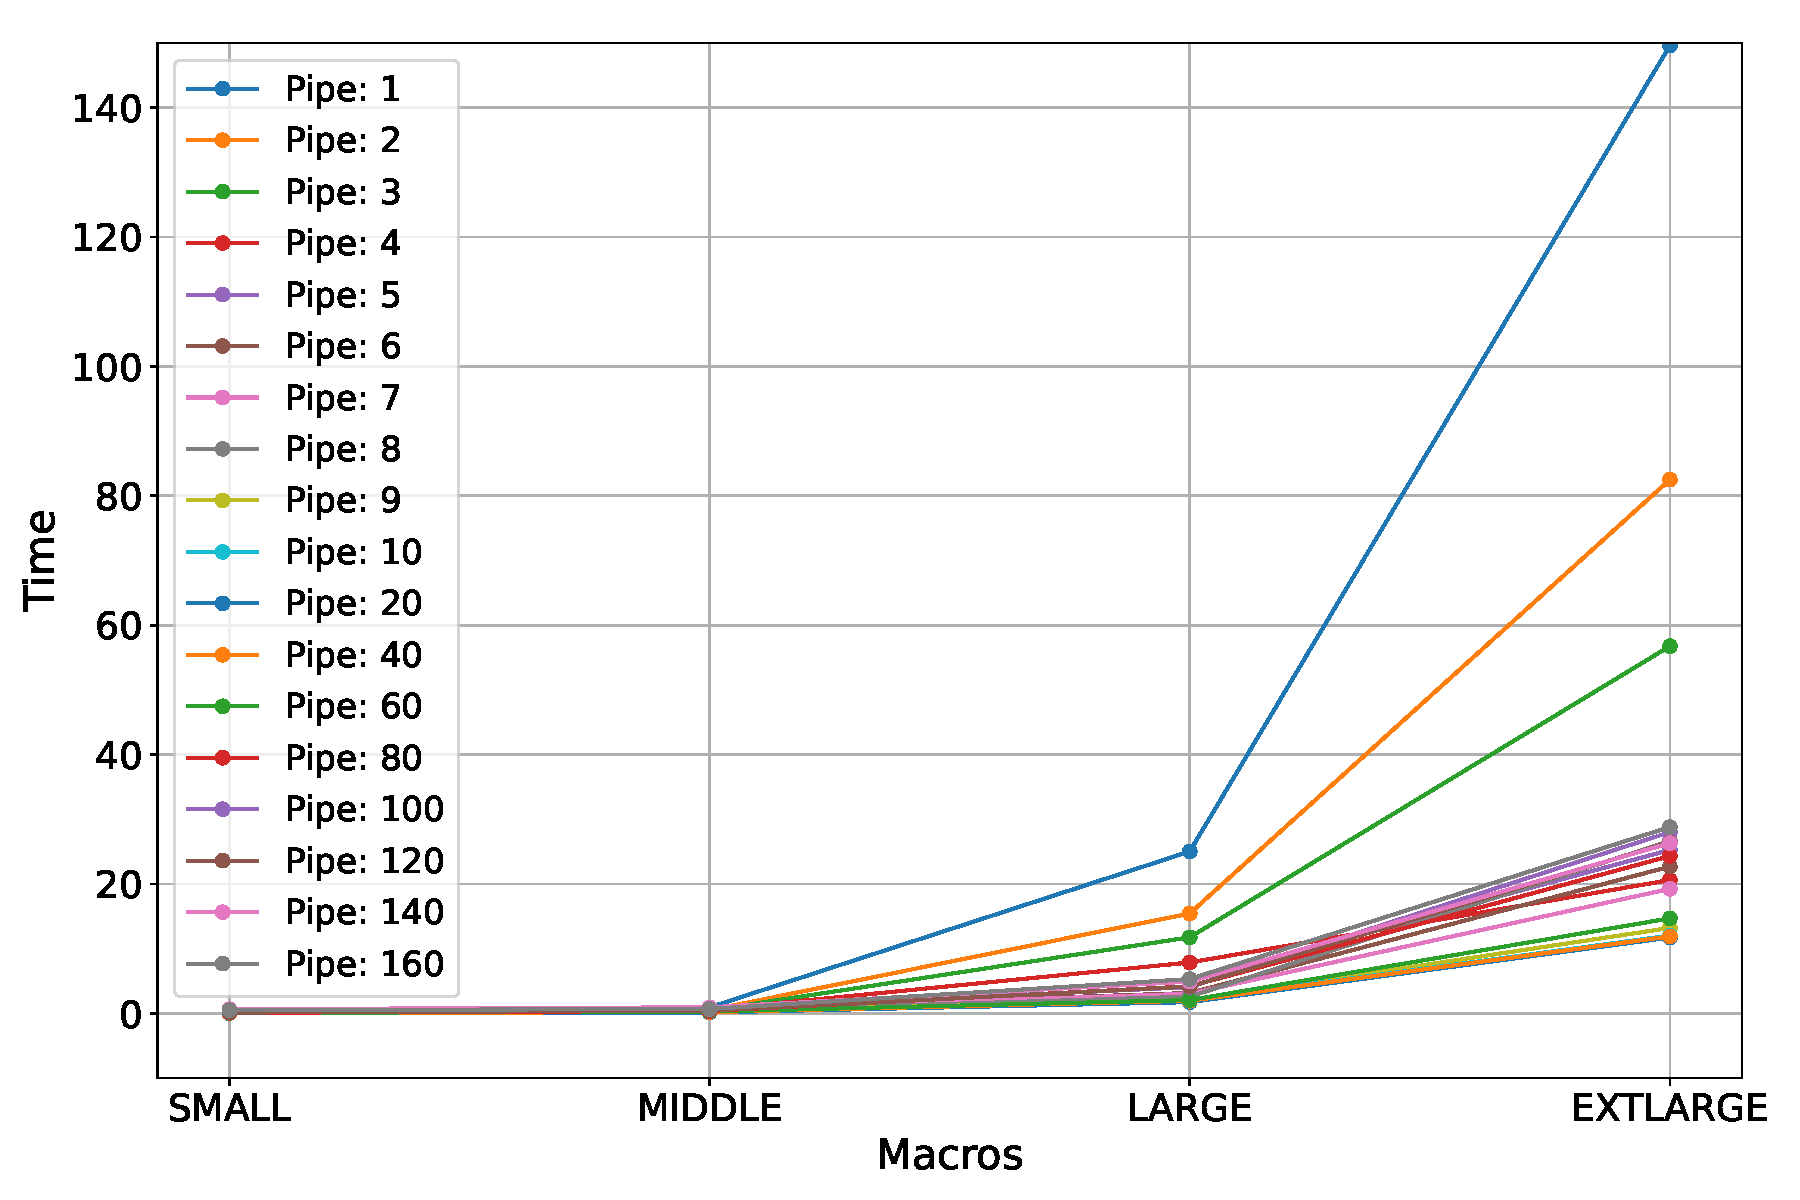
\includegraphics[width=0.6\textwidth]{../graph/for1.pdf} \\
    \small \it
    График 1.2\\ Графики 1.1, 1.2 --- Зависимость времени работы программы от объема входных данных и количества потоков при оптимизации с помощью директивы \texttt{for}.
\end{center}

\begin{center}
    \begin{tabular}{l | l l l l l l l l l}
        & \texttt{1} & \texttt{2} & \texttt{3} & \texttt{4} & \texttt{5} & \texttt{6} & \texttt{7} & \texttt{8} & \texttt{9} \\
        \hline
        \texttt{SMALL}    & $0.11$ & $0.07$ & $0.06$ & $0.06$ & $0.08$ & $0.08$ & $0.05$ & $0.06$ & $0.05$ \\
        \texttt{MIDDLE}   & $0.93$ & $0.50$ & $0.44$ & $0.54$ & $0.57$ & $0.67$ & $0.57$ & $0.34$ & $0.36$ \\
        \texttt{LARGE}    & $25.03$ & $15.44$ & $11.76$ & $7.87$ & $5.08$ & $3.15$ & $3.04$ & $2.59$ & $2.01$ \\
        \texttt{EXTLARGE} & $149.6$ & $82.5$ & $56.76$ & $20.61$ & $25.27$ & $22.69$ & $19.25$ & $26.63$ & $13.21$ \\
        \vspace{0.4cm}\\
        & \texttt{10} & \texttt{20} & \texttt{40} & \texttt{60} & \texttt{80} & \texttt{100} & \texttt{120} & \texttt{140} & \texttt{160} \\
        \hline
        \texttt{SMALL}    & $0.07$ & $0.03$ & $0.05$ & $0.07$ & $0.09$ & $0.14$ & $0.12$ & $0.65$ & $0.50$ \\
        \texttt{MIDDLE}   & $0.30$ & $0.14$ & $0.20$ & $0.29$ & $0.38$ & $0.62$ & $0.43$ & $0.94$ & $0.68$ \\
        \texttt{LARGE}    & $1.80$ & $1.74$ & $1.95$ & $2.05$ & $4.18$ & $4.06$ & $4.15$ & $4.91$ & $5.31$ \\
        \texttt{EXTLARGE} & $12.02$ & $11.72$ & $11.90$ & $14.69$ & $24.32$ & $28.01$ & $26.45$ & $26.32$ & $28.81$ \\
    \end{tabular}\\
    \vspace{0.3cm}
    \small \it
    Таблица 1. Результаты оптимизации с помощью директивы \texttt{for}. Значения указаны в секундах и округлены до сотых.
\end{center}
\newpage

\subsubsection*{Тестирование программы на Polus. Флаг оптимизации \texttt{-O2}}
\addcontentsline{toc}{subsubsection}{Тестирование программы на Polus. Флаг оптимизации \texttt{-O2}}
\begin{center}
    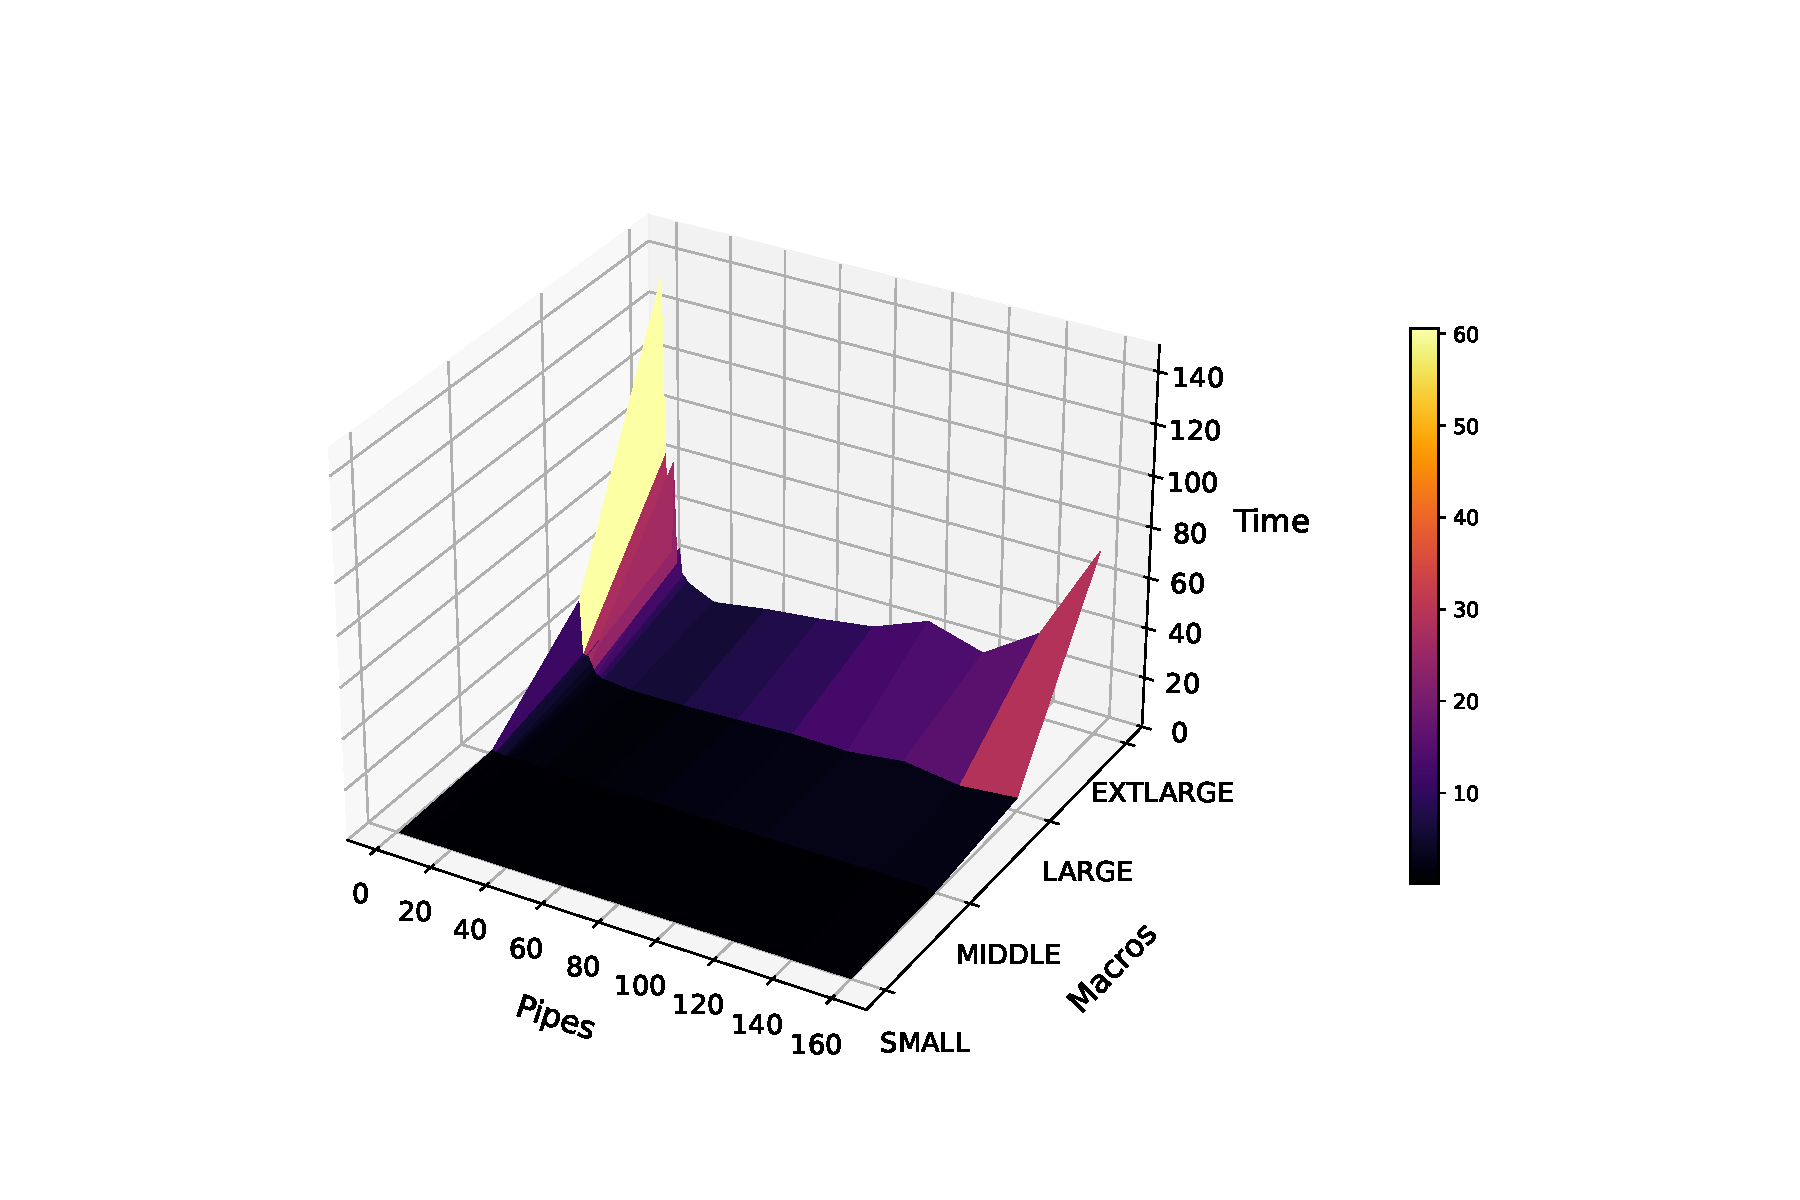
\includegraphics[width=0.8\textwidth]{../graph/for_o2.pdf} \\
    \small \it
    График 2.1
\end{center}

\begin{center}
    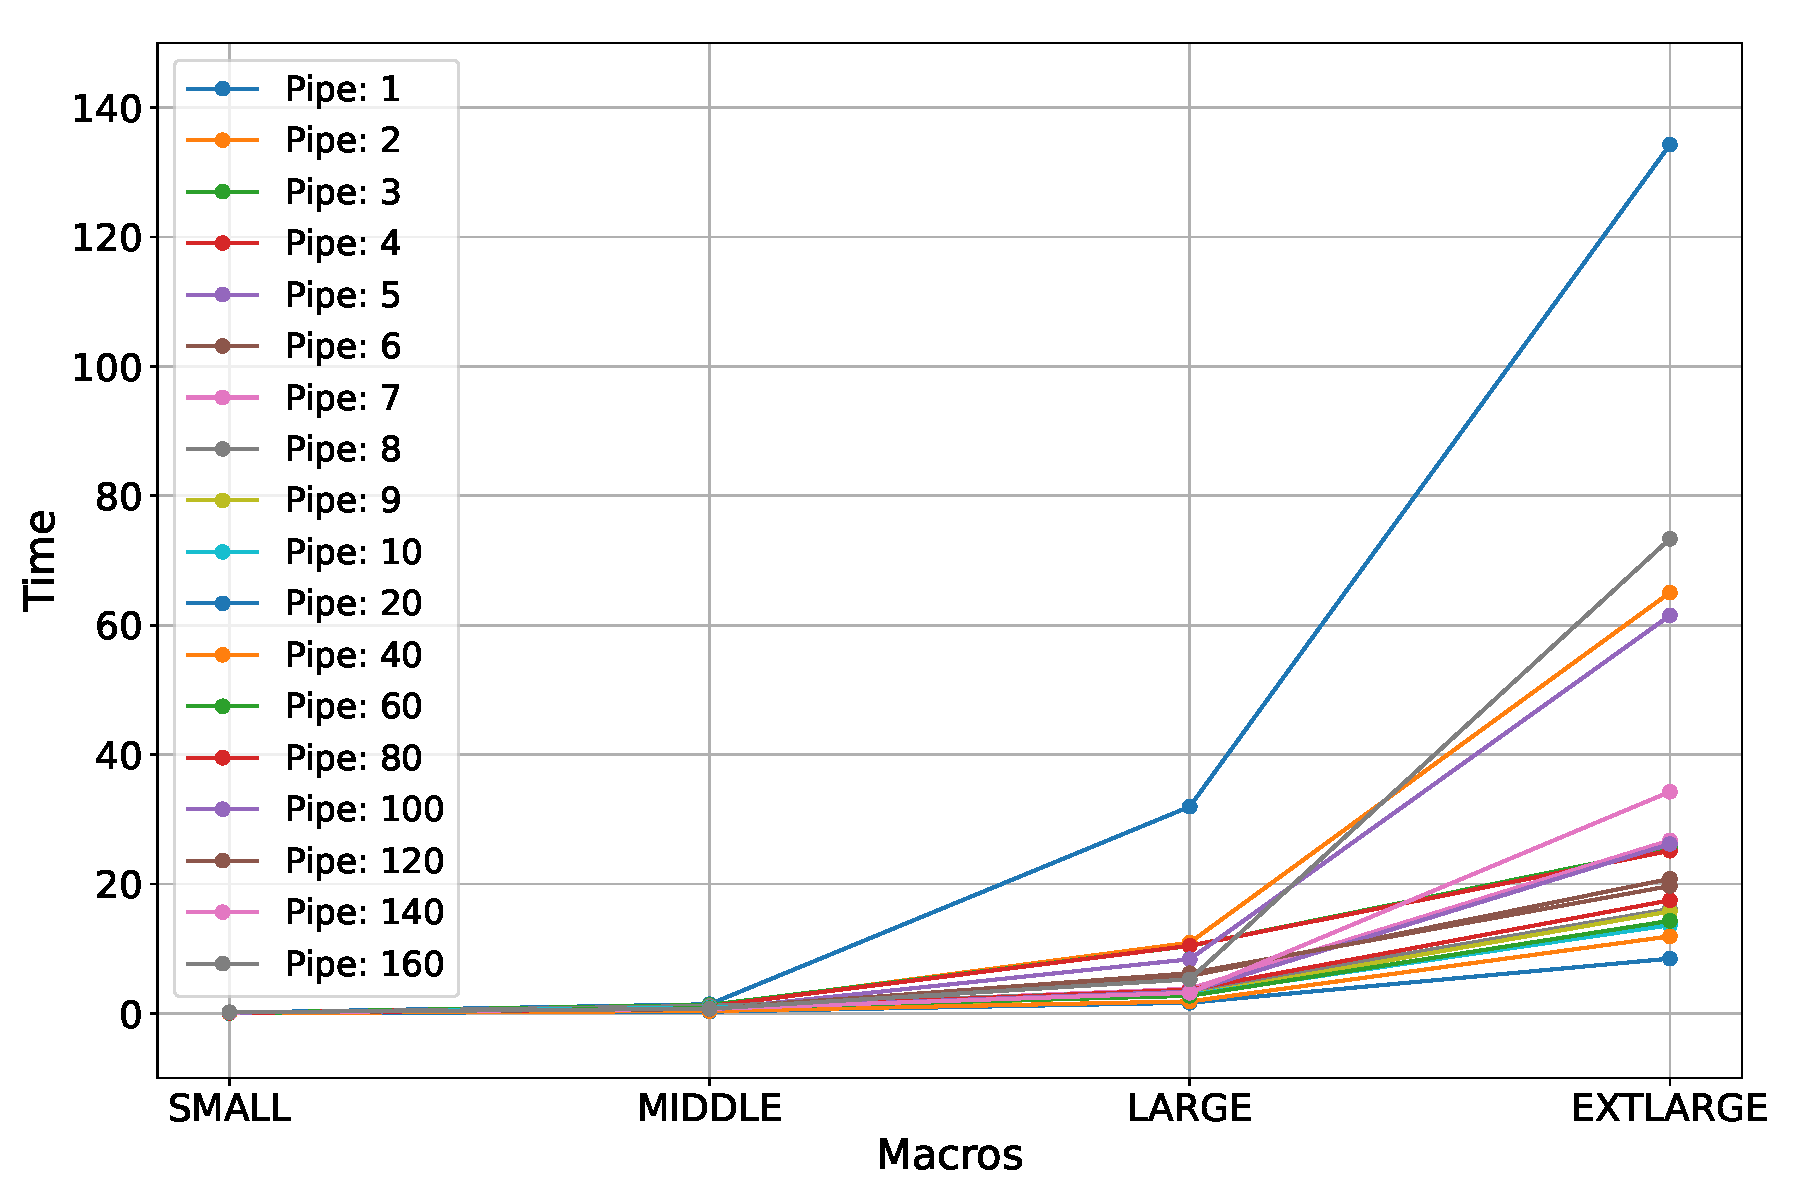
\includegraphics[width=0.6\textwidth]{../graph/for_o21.pdf} \\
    \small \it
    График 2.2\\ Графики 2.1, 2.2 --- Зависимость времени работы программы от объема входных данных и количества потоков при оптимизации с помощью директивы \texttt{for} и флага \texttt{-O2}.
\end{center}

\begin{center}
    \begin{tabular}{l | l l l l l l l l l}
        & \texttt{1} & \texttt{2} & \texttt{3} & \texttt{4} & \texttt{5} & \texttt{6} & \texttt{7} & \texttt{8} & \texttt{9} \\
        \hline
        \texttt{SMALL}    & $0.11$ & $0.10$ & $0.08$ & $0.09$ & $0.09$ & $0.08$ & $0.09$ & $0.05$ & $0.06$ \\
        \texttt{MIDDLE}   & $1.41$ & $1.15$ & $1.31$ & $1.12$ & $0.59$ & $0.87$ & $0.77$ & $1.16$ & $0.44$ \\
        \texttt{LARGE}    & $31.95$ & $10.93$ & $10.43$ & $10.45$ & $8.37$ & $5.77$ & $3.82$ & $3.53$ & $2.84$ \\
        \texttt{EXTLARGE} & $134.27$ & $65.04$ & $25.57$ & $25.14$ & $61.51$ & $20.80$ & $26.74$ & $16.14$ & $15.77$ \\
        \vspace{0.4cm}\\
        & \texttt{10} & \texttt{20} & \texttt{40} & \texttt{60} & \texttt{80} & \texttt{100} & \texttt{120} & \texttt{140} & \texttt{160} \\
        \hline
        \texttt{SMALL}    & $0.06$ & $0.03$ & $0.04$ & $0.07$ & $0.09$ & $0.12$ & $0.13$ & $0.13$ & $0.18$ \\
        \texttt{MIDDLE}   & $0.89$ & $0.26$ & $0.36$ & $0.80$ & $0.68$ & $0.68$ & $0.66$ & $0.70$ & $0.72$ \\
        \texttt{LARGE}    & $1.64$ & $1.86$ & $2.71$ & $3.67$ & $3.38$ & $6.21$ & $3.19$ & $5.26$ & $2.85$ \\
        \texttt{EXTLARGE} & $8.46$ & $11.91$ & $14.30$ & $17.48$ & $26.18$ & $19.69$ & $34.25$ & $73.35$ & $16.14$ \\
    \end{tabular}\\
    \vspace{0.3cm}
    \small \it
    Таблица 2. Результаты оптимизации с помощью директивы \texttt{for} и флага \texttt{-O2}. Значения указаны в секундах и округлены до сотых.
\end{center}
\newpage

\subsubsection*{Тестирование программы на Polus. Флаг оптимизации \texttt{-O3}}
\addcontentsline{toc}{subsubsection}{Тестирование программы на Polus. Флаг оптимизации \texttt{-O3}}
\begin{center}
    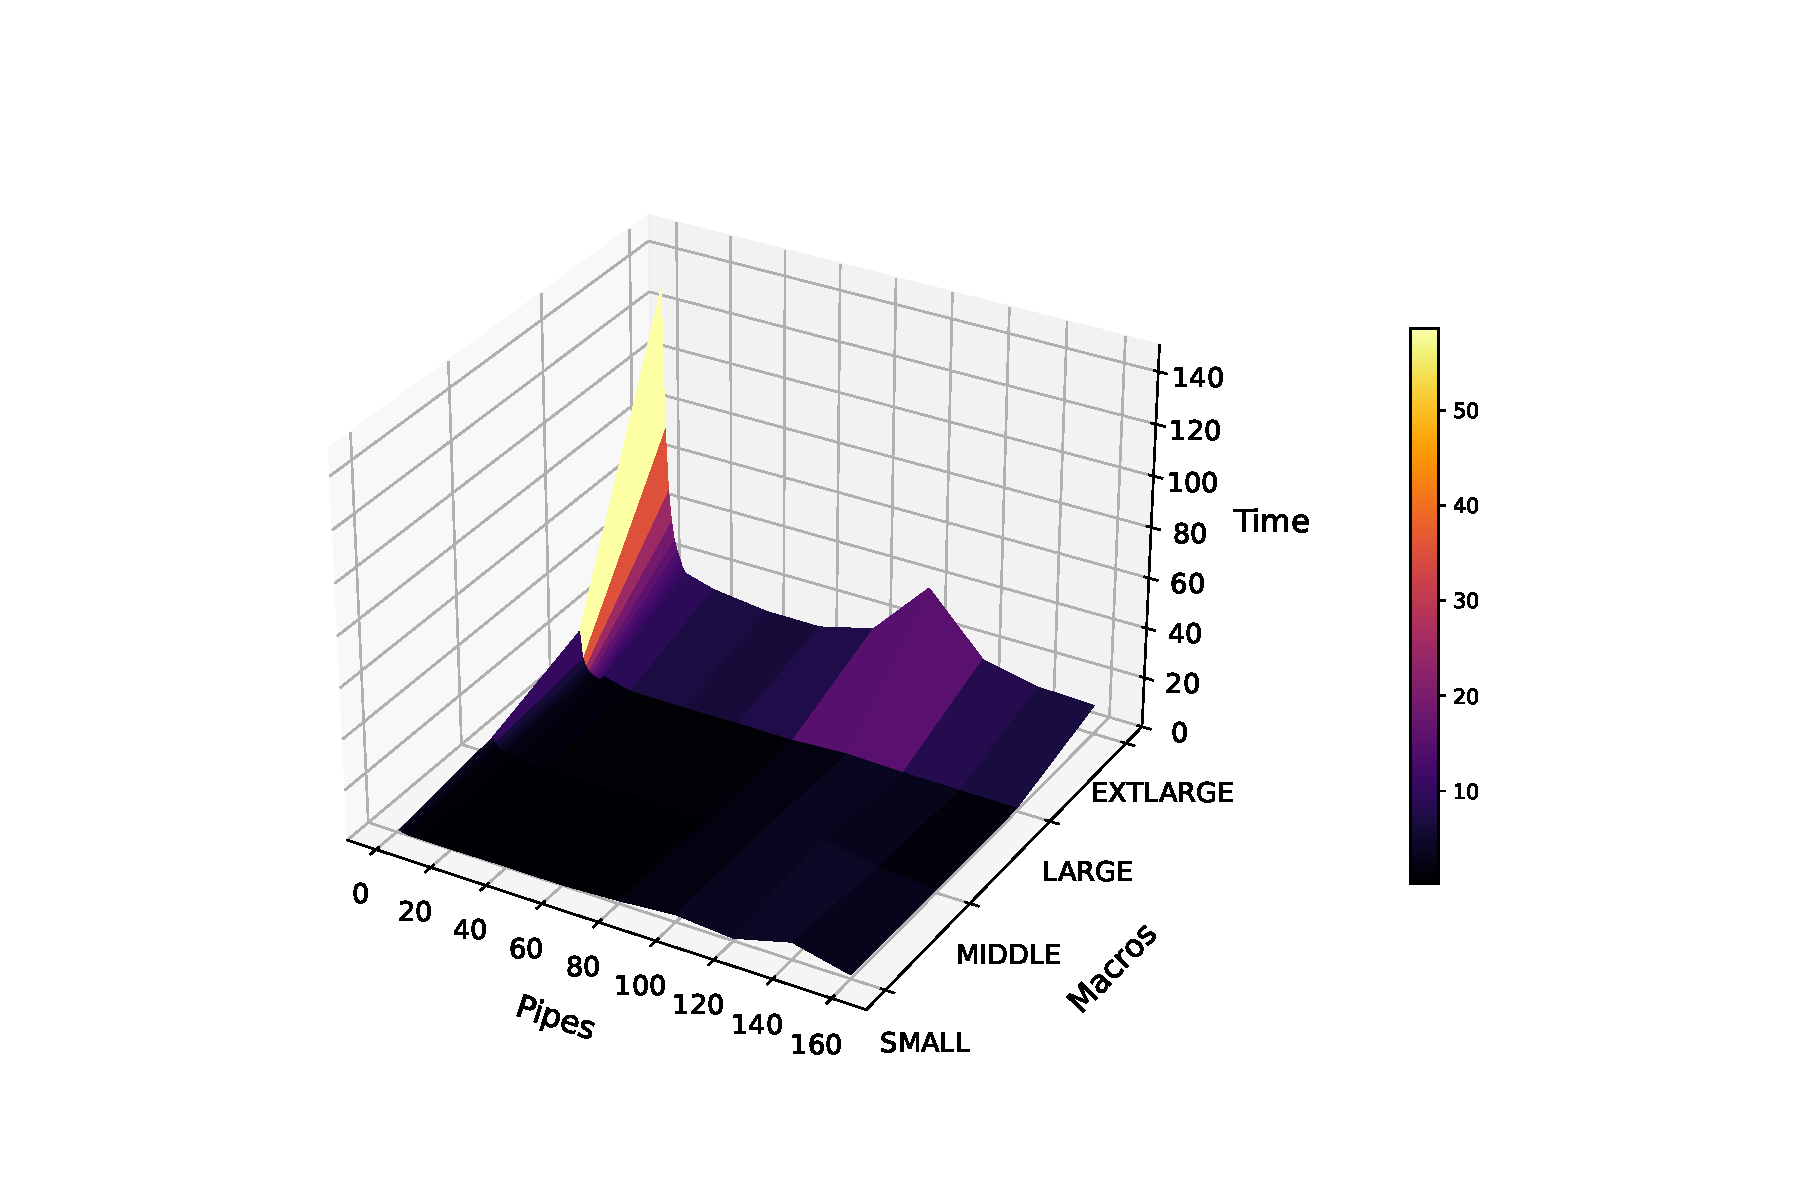
\includegraphics[width=0.8\textwidth]{../graph/for_o3.pdf} \\
    \small \it
    График 3.1
\end{center}

\begin{center}
    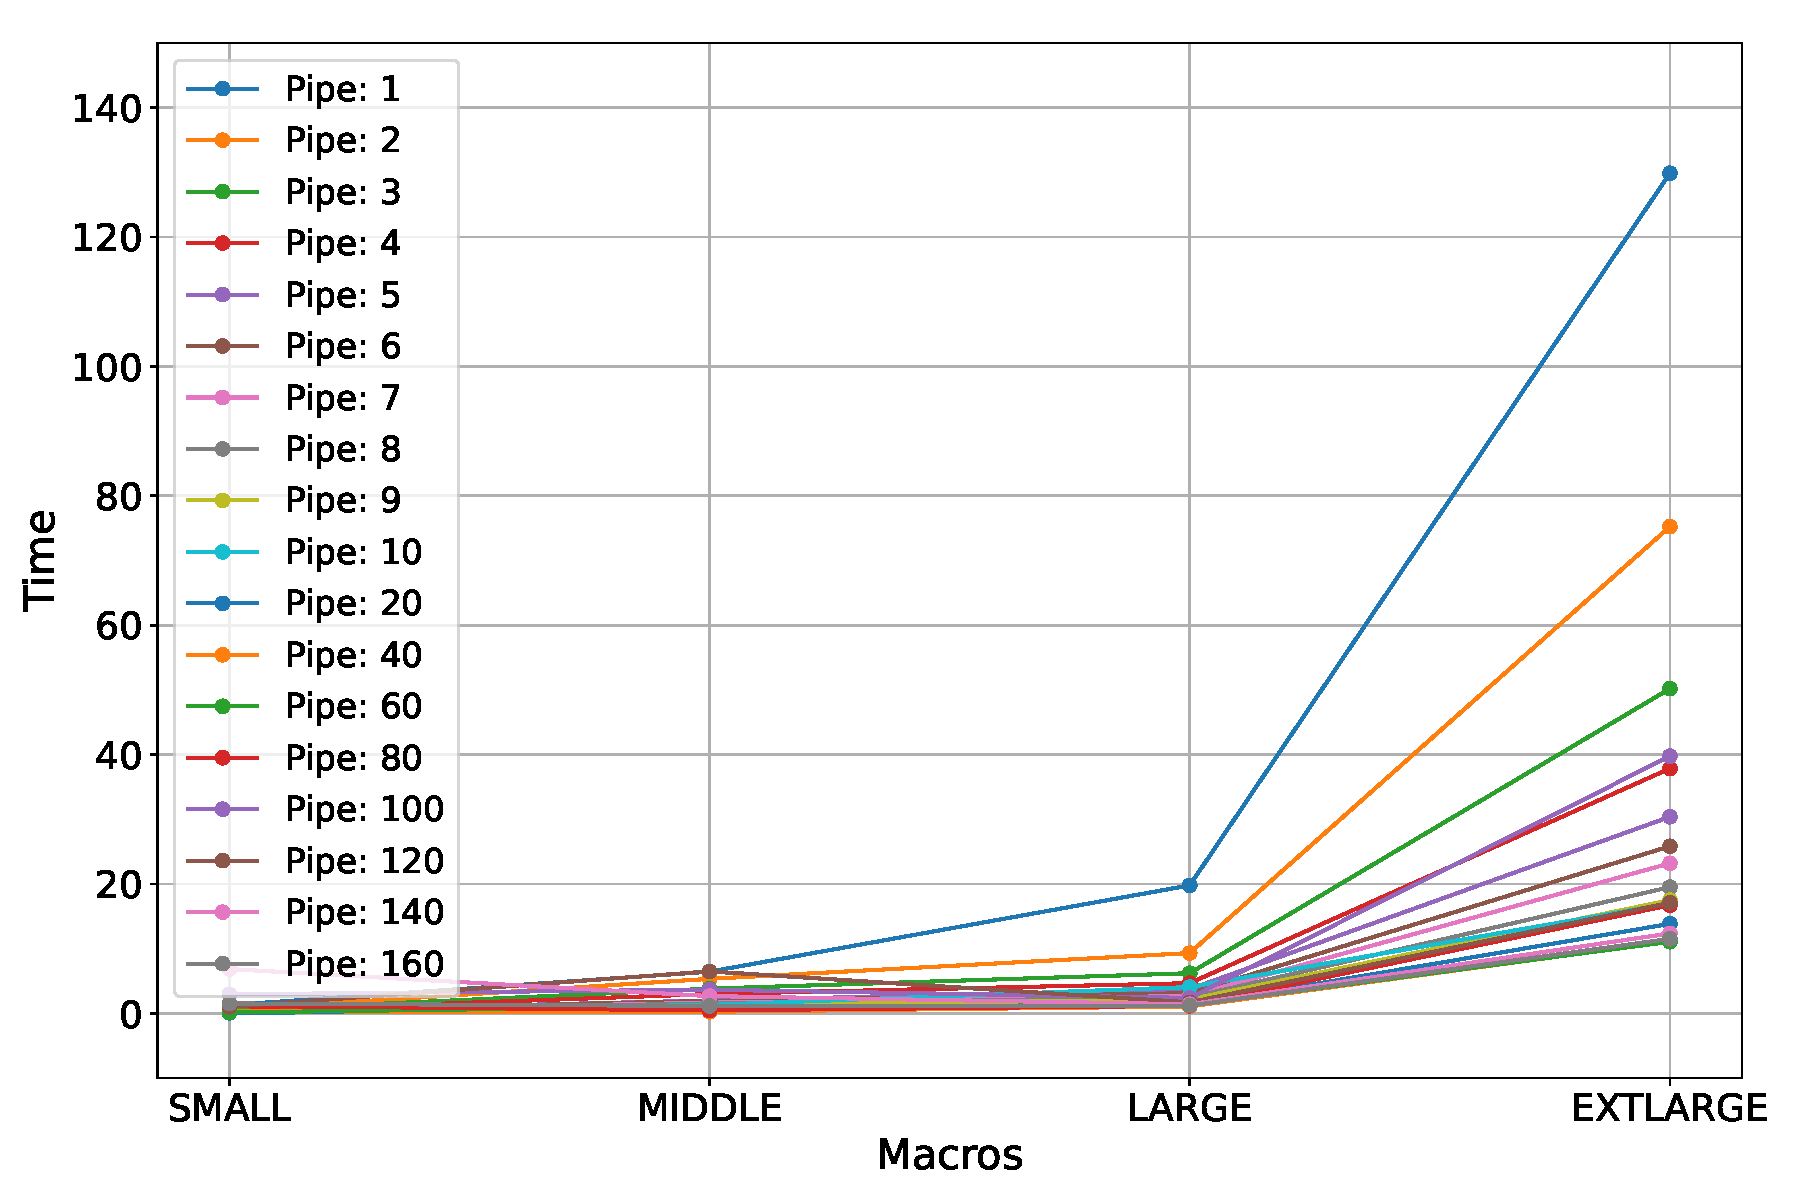
\includegraphics[width=0.6\textwidth]{../graph/for_o31.pdf} \\
    \small \it
    График 3.2\\ Графики 3.1, 3.2 --- Зависимость времени работы программы от объема входных данных и количества потоков при оптимизации с помощью директивы \texttt{for} и флага \texttt{-O3}.
\end{center}

\begin{center}
    \begin{tabular}{l | l l l l l l l l l}
        & \texttt{1} & \texttt{2} & \texttt{3} & \texttt{4} & \texttt{5} & \texttt{6} & \texttt{7} & \texttt{8} & \texttt{9} \\
        \hline
        \texttt{SMALL}    & $1.28$ & $0.56$ & $0.42$ & $0.32$ & $0.23$ & $0.25$ & $0.20$ & $0.19$ & $0.17$ \\
        \texttt{MIDDLE}   & $6.44$ & $5.34$ & $3.82$ & $2.99$ & $2.00$ & $1.93$ & $1.65$ & $1.54$ & $1.24$ \\
        \texttt{LARGE}    & $19.78$ & $9.32$ & $6.21$ & $4.67$ & $3.74$ & $3.12$ & $2.69$ & $2.45$ & $2.16$ \\
        \texttt{EXTLARGE} & $129.85$ & $75.23$ & $50.19$ & $37.85$ & $30.39$ & $25.83$ & $23.19$ & $19.52$ & $17.49$ \\
        \vspace{0.4cm}\\
        & \texttt{10} & \texttt{20} & \texttt{40} & \texttt{60} & \texttt{80} & \texttt{100} & \texttt{120} & \texttt{140} & \texttt{160} \\
        \hline
        \texttt{SMALL}    & $0.16$ & $0.08$ & $0.31$ & $0.14$ & $1.17$ & $2.94$ & $1.02$ & $6.85$ & $1.54$ \\
        \texttt{MIDDLE}   & $1.31$ & $0.55$ & $0.26$ & $1.09$ & $0.46$ & $3.66$ & $6.49$ & $2.67$ & $1.14$ \\
        \texttt{LARGE}    & $4.07$ & $1.26$ & $1.07$ & $1.27$ & $1.17$ & $2.39$ & $1.70$ & $1.41$ & $1.19$ \\
        \texttt{EXTLARGE} & $17.00$ & $13.84$ & $11.13$ & $11.07$ & $16.72$ & $39.77$ & $17.10$ & $12.37$ & $11.52$ \\
    \end{tabular}\\
    \vspace{0.3cm}
    \small \it
    Таблица 3. Результаты оптимизации с помощью директивы \texttt{for} и флага \texttt{-O3}. Значения указаны в секундах и округлены до сотых.
\end{center}
\newpage

\subsection*{Параллелизация при помощи директивы \texttt{task}}
\addcontentsline{toc}{subsection}{Параллелизация при помощи директивы \texttt{task}}

\subsubsection*{Внесенные изменения}
\addcontentsline{toc}{subsubsection}{Внесенные изменения}
Для распараллеливания программы с использованием директивы \texttt{task} в программу были внесены следующие изменения:

\begin{itemize}
    \item Для параллелизации блоков кода используется директива \texttt{\#pragma omp parallel}, которая создает параллельную область, позволяя нескольким потокам работать одновременно. В частности, параллелизация применяется к циклам, выполняющим вычисления.
    \item Внутри параллельных областей используются директивы \texttt{\#pragma omp task} для параллельного выполнения отдельных итераций вложенных циклов. Это позволяет создать асинхронные задачи, которые выполняются одновременно в разных потоках.
    \item Для подсчета переменной \texttt{gosa} используется директива \texttt{atomic} для предотвращения гонок данных при добавлении локального значения к глобальной переменной. Это гарантирует корректную агрегацию результатов из разных потоков.
    \item Директива \texttt{firstprivate(\ldots)} применяется к переменным индексов \texttt{i}, \texttt{j}, \texttt{k}, чтобы обеспечить их локальные копии для каждого потока. Это предотвращает возможные проблемы с синхронизацией при параллельной обработке этих переменных.
    \item Директива \texttt{\#pragma omp taskwait} используется, чтобы гарантировать завершение всех асинхронных задач перед продолжением вычислений.
    \item Используется директива \texttt{shared} для массивов, которые должны быть доступны для всех потоков, и директива \texttt{private} для переменных, которые должны быть локальными для каждого потока.
\end{itemize}
\newpage

\subsubsection*{Код программы}
\addcontentsline{toc}{subsubsection}{Код программы}

\begin{lstlisting}
#include <omp.h>
#include <stdio.h>

#define LARGE

#ifdef SMALL
#define MIMAX 65
#define MJMAX 33
#define MKMAX 33
#endif

#ifdef MIDDLE
#define MIMAX 129
#define MJMAX 65
#define MKMAX 65
#endif

#ifdef LARGE
#define MIMAX 257
#define MJMAX 129
#define MKMAX 129
#endif

#ifdef EXTLARGE
#define MIMAX 513
#define MJMAX 257
#define MKMAX 257
#endif

#define NN 200

static float a[MIMAX][MJMAX][MKMAX][4],
             b[MIMAX][MJMAX][MKMAX][3], c[MIMAX][MJMAX][MKMAX][3];
static float p[MIMAX][MJMAX][MKMAX];
static float wrk1[MIMAX][MJMAX][MKMAX], wrk2[MIMAX][MJMAX][MKMAX];
static float bnd[MIMAX][MJMAX][MKMAX];

static int imax, jmax, kmax;
static float omega;


void
initmt()
{
    int i, j, k;
    
    for (i = 0; i < imax; ++i) {
#pragma omp task firstprivate(i) private(j, k) shared(a, b, c, p, wrk1, bnd)
        {
            for (j = 0; j < jmax; ++j) {
                for (k = 0; k < kmax; ++k) {
                    a[i][j][k][0] = 0.0;
                    a[i][j][k][1] = 0.0;
                    a[i][j][k][2] = 0.0;
                    a[i][j][k][3] = 0.0;
                    b[i][j][k][0] = 0.0;
                    b[i][j][k][1] = 0.0;
                    b[i][j][k][2] = 0.0;
                    c[i][j][k][0] = 0.0;
                    c[i][j][k][1] = 0.0;
                    c[i][j][k][2] = 0.0;
                    p[i][j][k] = 0.0;
                    wrk1[i][j][k] = 0.0;
                    bnd[i][j][k] = 0.0;
                }
            }
        }
    }

    for (i = 0; i < imax; ++i) {
#pragma omp task firstprivate(i) private(j, k) shared(a, b, c, p, wrk1, bnd)
        {
            for (j = 0; j < jmax; ++j) {
                for (k = 0; k < kmax; ++k) {
                    a[i][j][k][0] = 1.0;
                    a[i][j][k][1] = 1.0;
                    a[i][j][k][2] = 1.0;
                    a[i][j][k][3] = 1.0 / 6.0;
                    c[i][j][k][0] = 1.0;
                    c[i][j][k][1] = 1.0;
                    c[i][j][k][2] = 1.0;
                    p[i][j][k] = (float) (k * k) /
                                 (float) ((kmax - 1) * (kmax - 1));
                    wrk1[i][j][k] = 0.0;
                    bnd[i][j][k] = 1.0;
                }
            }
        }
    }
}

float
jacobi(int nn)
{
    int i, j, k, n;
    float gosa;
    float s0, ss;
    float local_gosa = 0.0;

#pragma omp parallel shared(a, b, c, p, wrk1, wrk2, bnd, omega, gosa)
    {
#pragma omp single
        {
            for (n = 0; n < nn; ++n) {
                gosa = 0.0;
                for (i = 1; i < imax - 1; ++i) {
#pragma omp task firstprivate(i) private(s0, ss, local_gosa)
                    {
                        local_gosa = 0.0;

                        for (j = 1; j < jmax - 1; ++j) {
                            for (k = 1; k < kmax - 1; ++k) {
                                s0 = a[i][j][k][0] * p[i + 1][j][k] +
                                     a[i][j][k][1] * p[i][j + 1][k] +
                                     a[i][j][k][2] * p[i][j][k + 1] +
                                     b[i][j][k][0] * (p[i + 1][j + 1][k] -
                                                      p[i + 1][j - 1][k] -
                                                      p[i - 1][j + 1][k] +
                                                      p[i - 1][j - 1][k]) +
                                     b[i][j][k][1] * (p[i][j + 1][k + 1] -
                                                      p[i][j - 1][k + 1] -
                                                      p[i][j + 1][k - 1] +
                                                      p[i][j - 1][k - 1]) +
                                     b[i][j][k][2] * (p[i + 1][j][k + 1] -
                                                      p[i - 1][j][k + 1] -
                                                      p[i + 1][j][k - 1] +
                                                      p[i - 1][j][k - 1]) +
                                     c[i][j][k][0] * p[i - 1][j][k] +
                                     c[i][j][k][1] * p[i][j - 1][k] +
                                     c[i][j][k][2] * p[i][j][k - 1] +
                                     wrk1[i][j][k];


                                ss = (s0 * a[i][j][k][3] - p[i][j][k]) *
                                      bnd[i][j][k];
                                local_gosa += ss * ss;

                                wrk2[i][j][k] = p[i][j][k] + omega * ss;
                            }
                        }
#pragma omp atomic
                    gosa += local_gosa;
#pragma omp taskwait
                    }
               }

                for (i = 1; i < imax - 1; ++i) {
#pragma omp task firstprivate(i)
                    for (j = 1; j < jmax - 1; ++j) {
                        for (k = 1; k < kmax - 1; ++k)
                            p[i][j][k] = wrk2[i][j][k];
                    }
#pragma omp taskwait
                }
            }
        }
    }

    return gosa;
}

int
main()
{
    int i, j, k;
    float gosa;
    double cpu0, cpu1, cpu2, cpu3, nflop, xmflops2, score;

    omega = 0.8;
    imax = MIMAX - 1;
    jmax = MJMAX - 1;
    kmax = MKMAX - 1;

    cpu2 = omp_get_wtime();
    
    initmt();
    
    cpu3 = omp_get_wtime();
    
    printf("mimax = %d mjmax = %d mkmax = %d\n", MIMAX, MJMAX, MKMAX);
    printf("imax = %d jmax = %d kmax =%d\n", imax, jmax, kmax);


    cpu0 = omp_get_wtime();

    gosa = jacobi(NN);

    cpu1 = omp_get_wtime();

    nflop = (kmax - 2) * (jmax - 2) * (imax - 2) * 34;

    if (cpu1 != 0.0) {
        xmflops2 = nflop / cpu1 * 1.0e-6 * (float) NN;
    }

    score = xmflops2 / 32.27;

    printf("cpu : %f sec.\n", cpu1 - cpu0);
    printf("init : %f sec.\n", cpu3 - cpu2);
    printf("Loop executed for %d times\n", NN);
    printf("Gosa : %e \n", gosa);
    printf("MFLOPS measured : %f\n", xmflops2);
    printf("Score based on MMX Pentium 200MHz : %f\n", score);
    printf("\n");

    return (0);
}
\end{lstlisting}
\newpage

\subsubsection*{Тестирование программы на Polus}
\addcontentsline{toc}{subsubsection}{Тестирование программы на Polus}
\begin{center}
    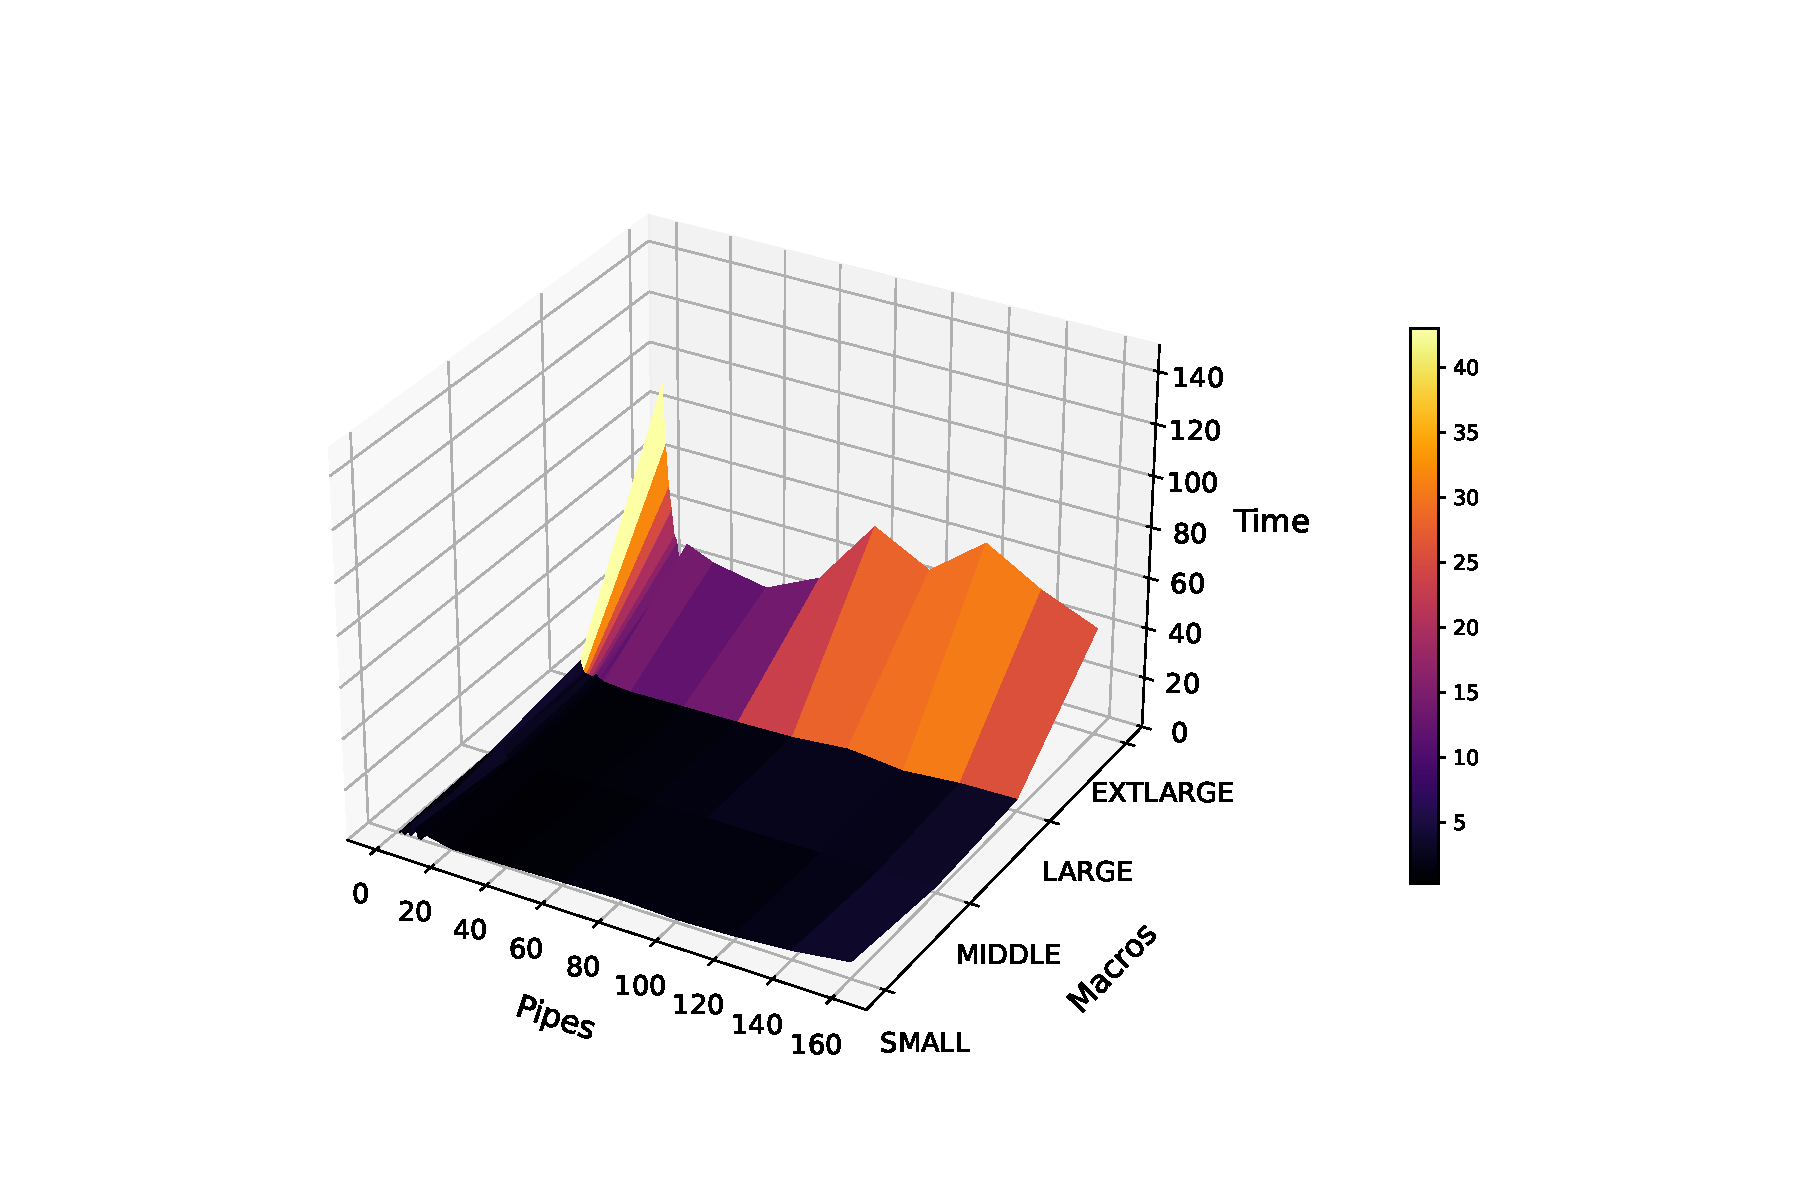
\includegraphics[width=0.8\textwidth]{../graph/task.pdf} \\
    \small \it
    График 4.1
\end{center}

\begin{center}
    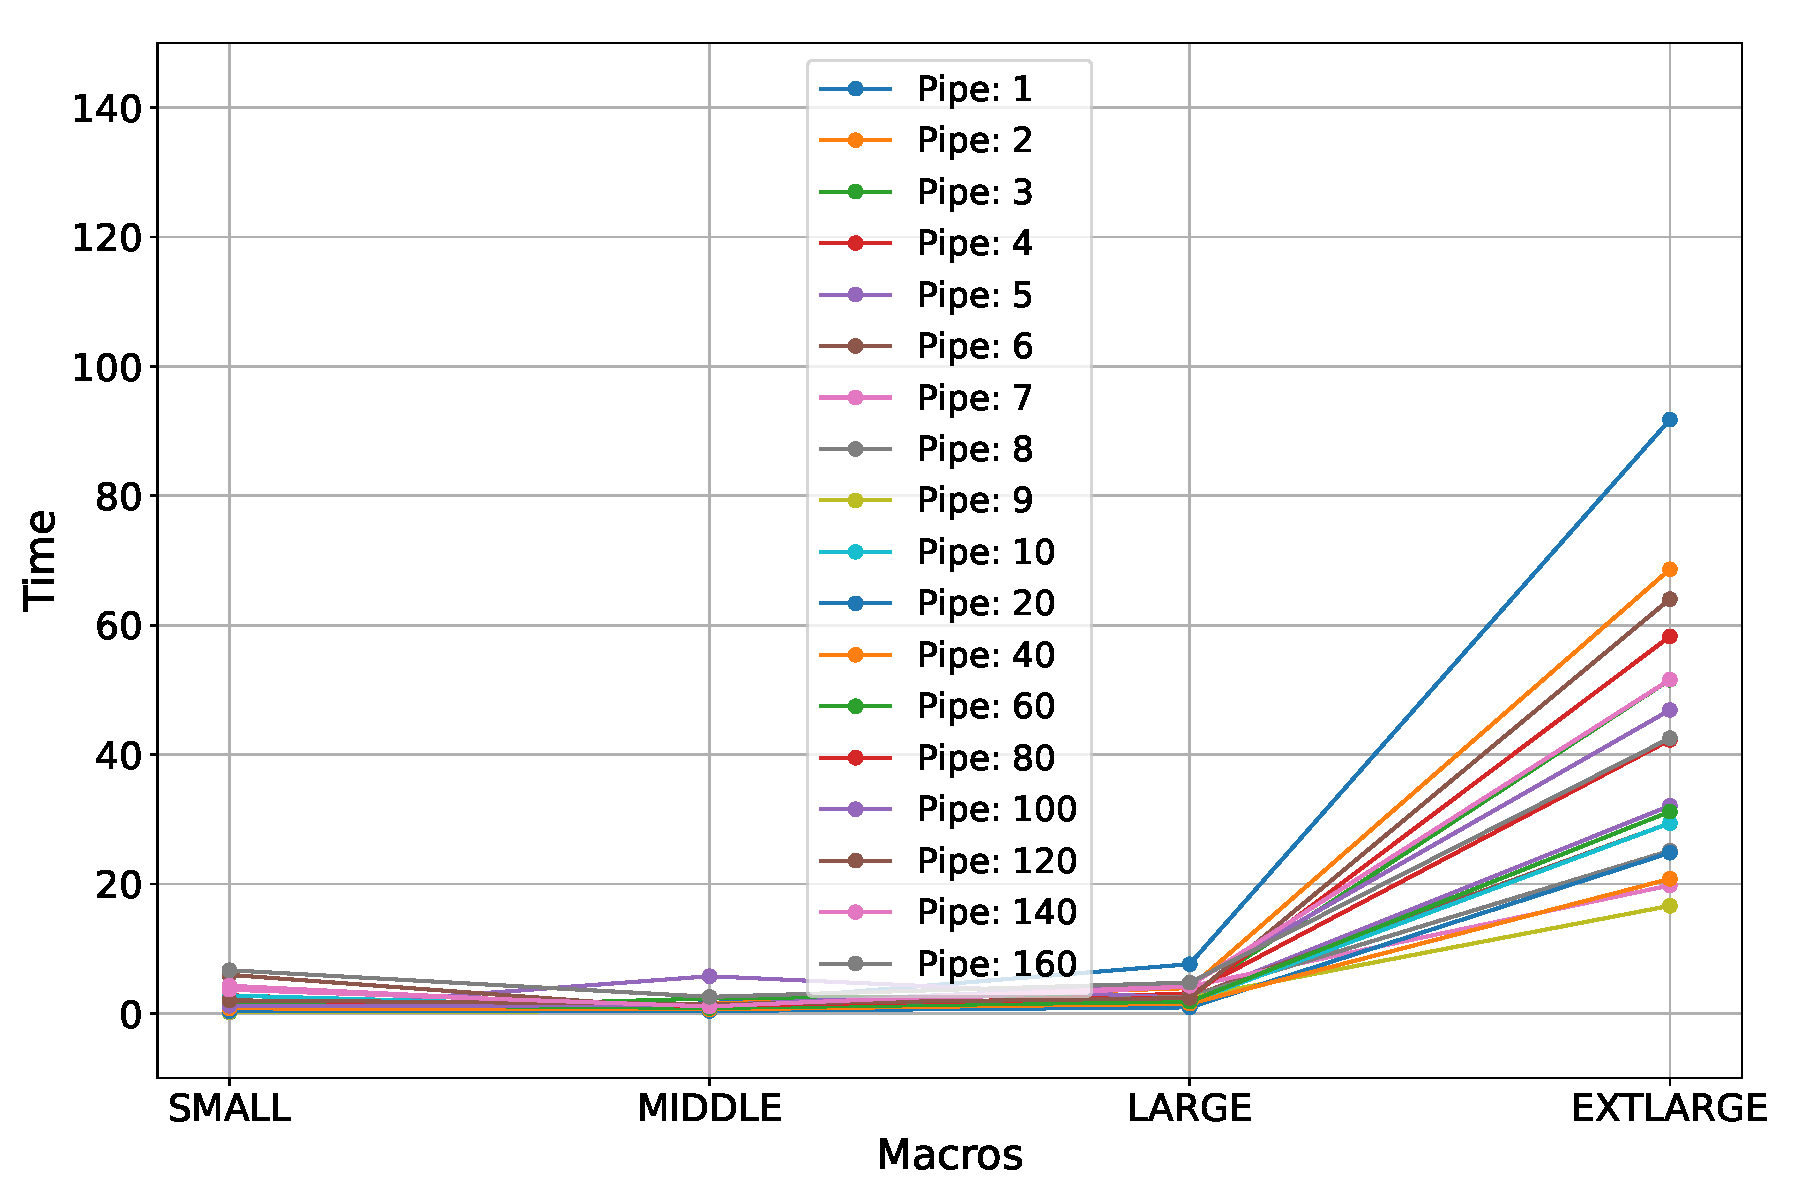
\includegraphics[width=0.6\textwidth]{../graph/task1.pdf} \\
    \small \it
    График 4.2\\ Графики 4.1, 4.2 --- Зависимость времени работы программы от объема входных данных и количества потоков при оптимизации с помощью директивы \texttt{task}.
\end{center}

\begin{center}
    \begin{tabular}{l | l l l l l l l l l}
        & \texttt{1} & \texttt{2} & \texttt{3} & \texttt{4} & \texttt{5} & \texttt{6} & \texttt{7} & \texttt{8} & \texttt{9} \\
        \hline
        \texttt{SMALL}    & $0.21$ & $0.79$ & $0.14$ & $2.8$ & $0.18$ & $5.96$ & $4.28$ & $0.24$ & $0.2$ \\
        \texttt{MIDDLE}   & $1.55$ & $1.5$ & $2.31$ & $0.43$ & $5.74$ & $0.49$ & $0.58$ & $0.41$ & $0.36$ \\
        \texttt{LARGE}    & $7.61$ & $3.91$ & $2.9$ & $3.1$ & $2.37$ & $2.51$ & $4.16$ & $2.59$ & $2.42$ \\
        \texttt{EXTLARGE} & $91.77$ & $68.64$ & $51.56$ & $42.26$ & $32.07$ & $29.4$ & $19.79$ & $25.13$ & $16.63$ \\
        \vspace{0.4cm}\\
        & \texttt{10} & \texttt{20} & \texttt{40} & \texttt{60} & \texttt{80} & \texttt{100} & \texttt{120} & \texttt{140} & \texttt{160} \\
        \hline
        \texttt{SMALL}    & $2.76$ & $0.34$ & $0.78$ & $1.4$ & $2.02$ & $1.18$ & $2.01$ & $3.66$ & $6.67$ \\
        \texttt{MIDDLE}   & $0.69$ & $0.37$ & $0.61$ & $0.83$ & $1.16$ & $1.25$ & $1.43$ & $1.07$ & $2.55$ \\
        \texttt{LARGE}    & $0.93$ & $1.5$ & $1.82$ & $2.45$ & $4.5$ & $2.36$ & $4.27$ & $4.76$ & $3.91$ \\
        \texttt{EXTLARGE} & $24.83$ & $20.79$ & $31.18$ & $58.26$ & $46.89$ & $64.03$ & $51.58$ & $42.55$ & $42.26$ \\
    \end{tabular}\\
    \vspace{0.3cm}
    \small \it
    Таблица 4. Результаты оптимизации с помощью директивы \texttt{task}. Значения указаны в секундах и округлены до сотых.  
\end{center}
\newpage

\subsubsection*{Тестирование программы на Polus. Флаг оптимизации \texttt{-O2}}
\addcontentsline{toc}{subsubsection}{Тестирование программы на Polus. Флаг оптимизации \texttt{-O2}}
\begin{center}
    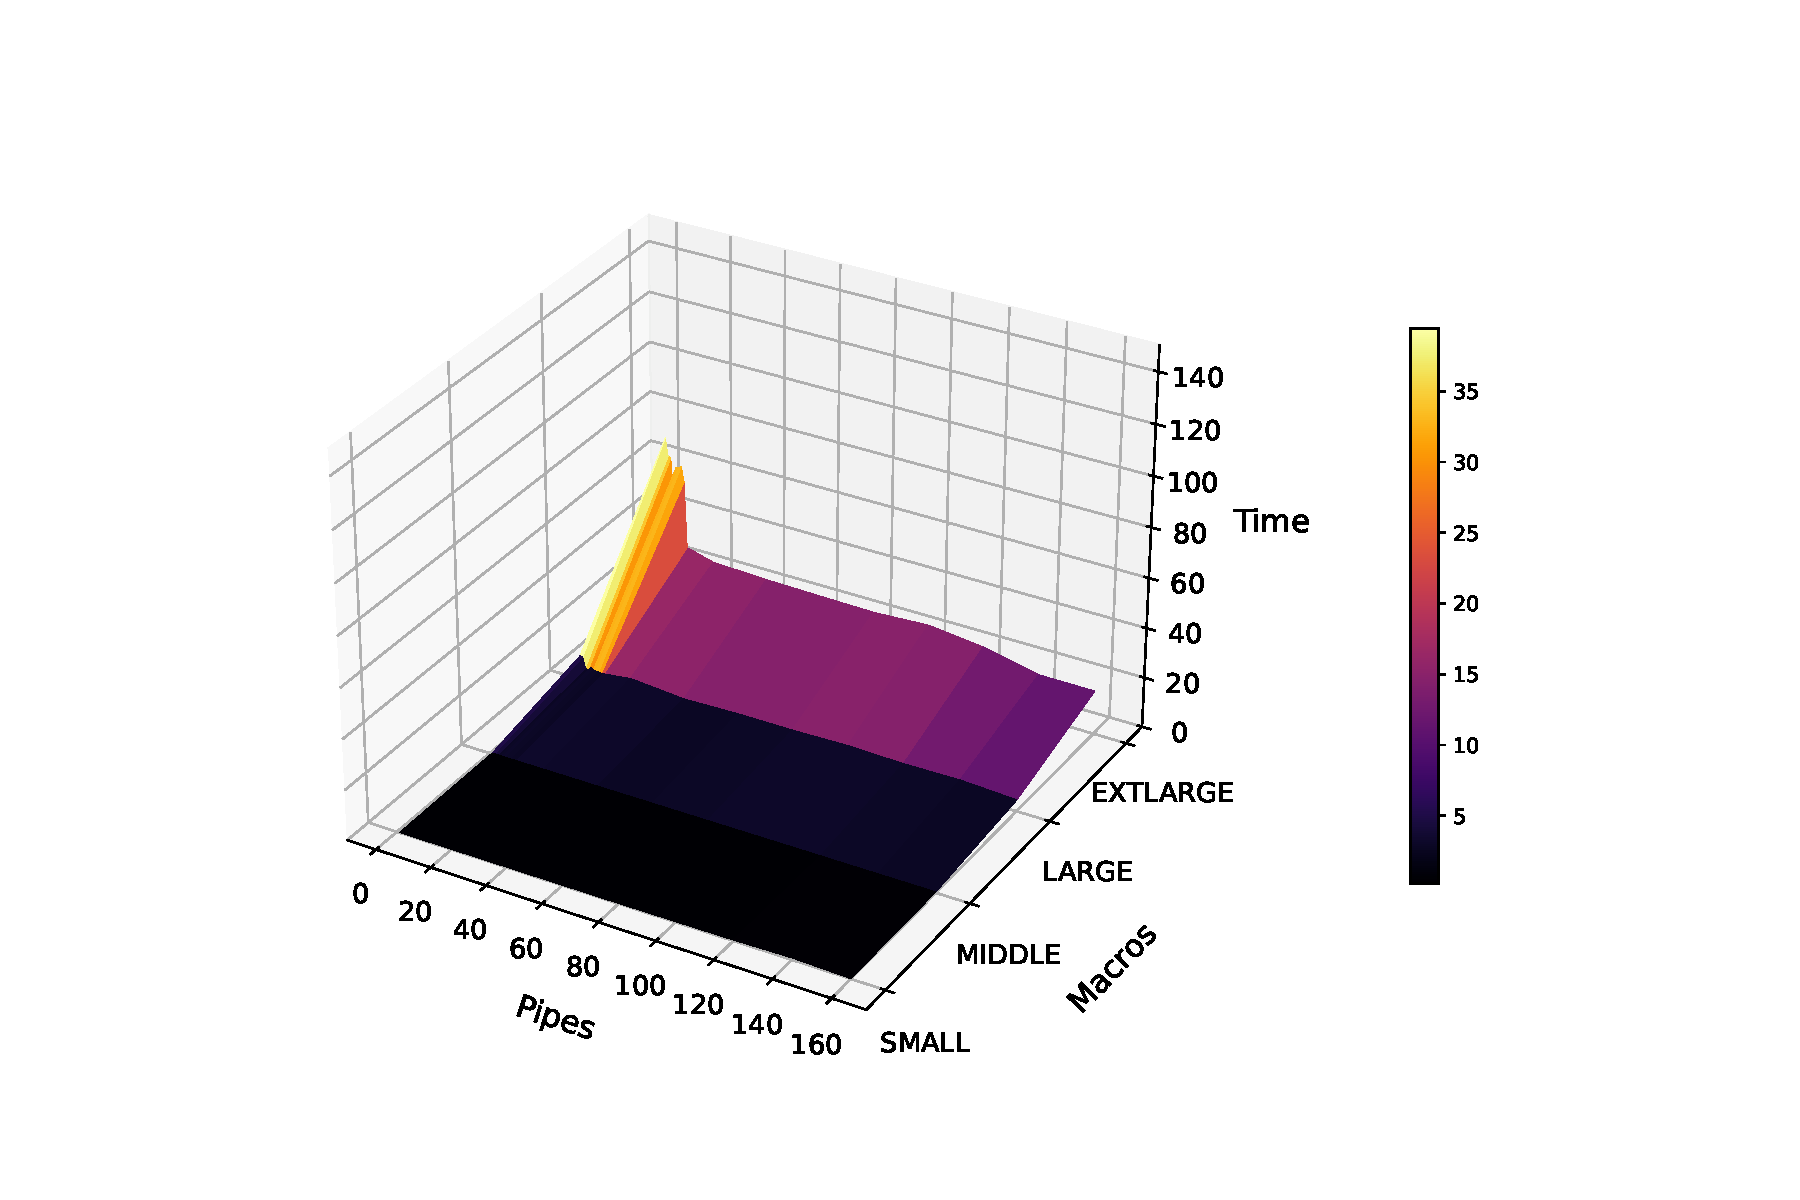
\includegraphics[width=0.8\textwidth]{../graph/task_o2.pdf} \\
    \small \it
    График 5.1
\end{center}

\begin{center}
    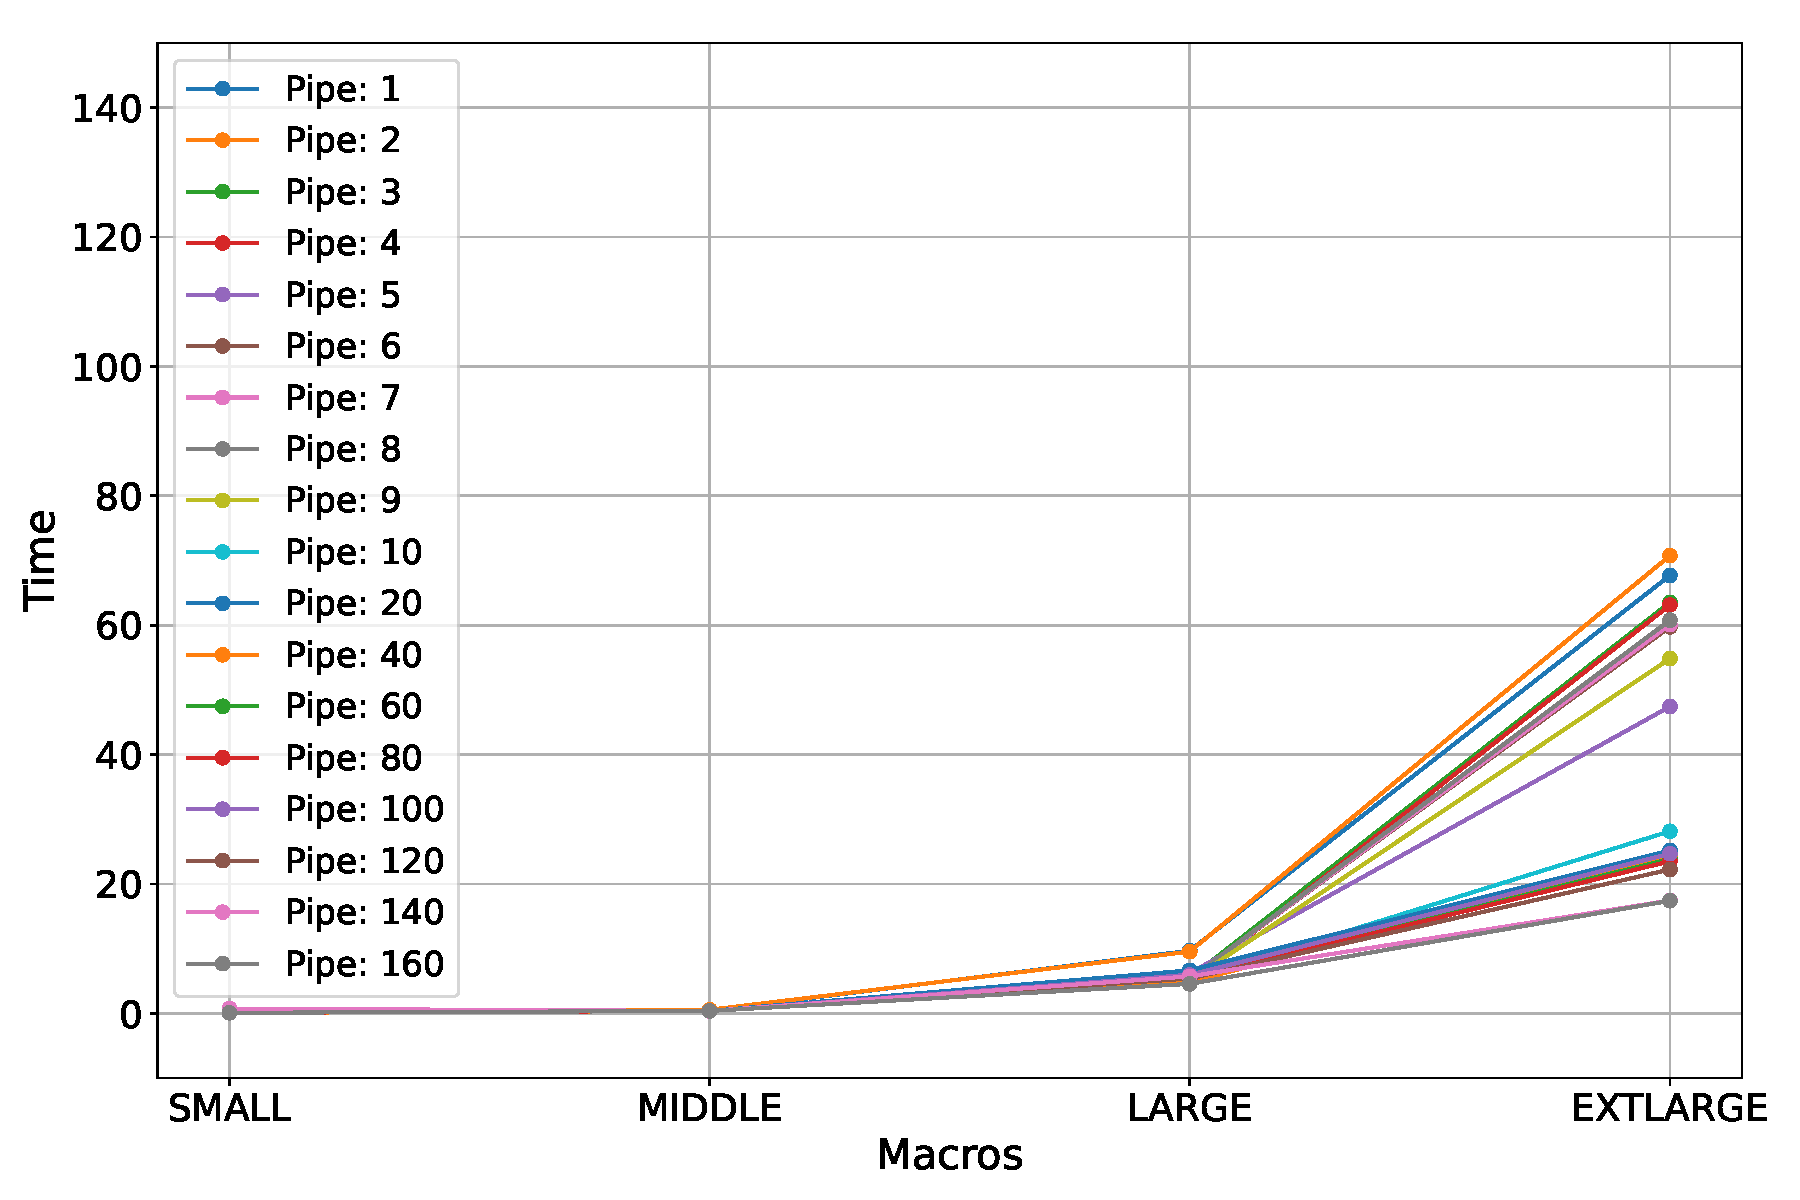
\includegraphics[width=0.6\textwidth]{../graph/task_o21.pdf} \\
    \small \it
    График 5.2\\ Графики 5.1, 5.2 --- Зависимость времени работы программы от объема входных данных и количества потоков при оптимизации с помощью директивы \texttt{task} и флага \texttt{-O2}.
\end{center}

\begin{center}
    \begin{tabular}{l | l l l l l l l l l}
        & \texttt{1} & \texttt{2} & \texttt{3} & \texttt{4} & \texttt{5} & \texttt{6} & \texttt{7} & \texttt{8} & \texttt{9} \\
        \hline
        \texttt{SMALL}    & $0.09$ & $0.09$ & $0.09$ & $0.09$ & $0.09$ & $0.09$ & $0.09$ & $0.09$ & $0.09$ \\
        \texttt{MIDDLE}   & $0.43$ & $0.55$ & $0.37$ & $0.37$ & $0.37$ & $0.37$ & $0.38$ & $0.37$ & $0.37$ \\
        \texttt{LARGE}    & $9.68$ & $9.55$ & $5.45$ & $4.75$ & $6.22$ & $5.35$ & $5.33$ & $5.32$ & $4.99$ \\
        \texttt{EXTLARGE} & $67.69$ & $70.74$ & $63.52$ & $63.11$ & $47.43$ & $59.73$ & $60.09$ & $60.78$ & $54.84$ \\
        \vspace{0.4cm}\\
        & \texttt{10} & \texttt{20} & \texttt{40} & \texttt{60} & \texttt{80} & \texttt{100} & \texttt{120} & \texttt{140} & \texttt{160} \\
        \hline
        \texttt{SMALL}    & $0.09$ & $0.09$ & $0.09$ & $0.09$ & $0.09$ & $0.19$ & $0.32$ & $0.75$ & $0.09$ \\
        \texttt{MIDDLE}   & $0.37$ & $0.37$ & $0.37$ & $0.38$ & $0.37$ & $0.37$ & $0.37$ & $0.37$ & $0.38$ \\
        \texttt{LARGE}    & $5.18$ & $6.65$ & $4.84$ & $5.43$ & $5.45$ & $5.94$ & $5.39$ & $5.72$ & $4.56$ \\
        \texttt{EXTLARGE} & $28.15$ & $25.18$ & $24.30$ & $23.87$ & $23.51$ & $24.68$ & $22.24$ & $17.44$ & $17.41$ \\
    \end{tabular}\\
    \vspace{0.3cm}
    \small \it
    Таблица 5. Результаты оптимизации с помощью директивы \texttt{task} и флага \texttt{-O2}. Значения указаны в секундах и округлены до сотых.
\end{center}
\newpage

\subsubsection*{Тестирование программы на Polus. Флаг оптимизации \texttt{-O3}}
\addcontentsline{toc}{subsubsection}{Тестирование программы на Polus. Флаг оптимизации \texttt{-O3}}
\begin{center}
    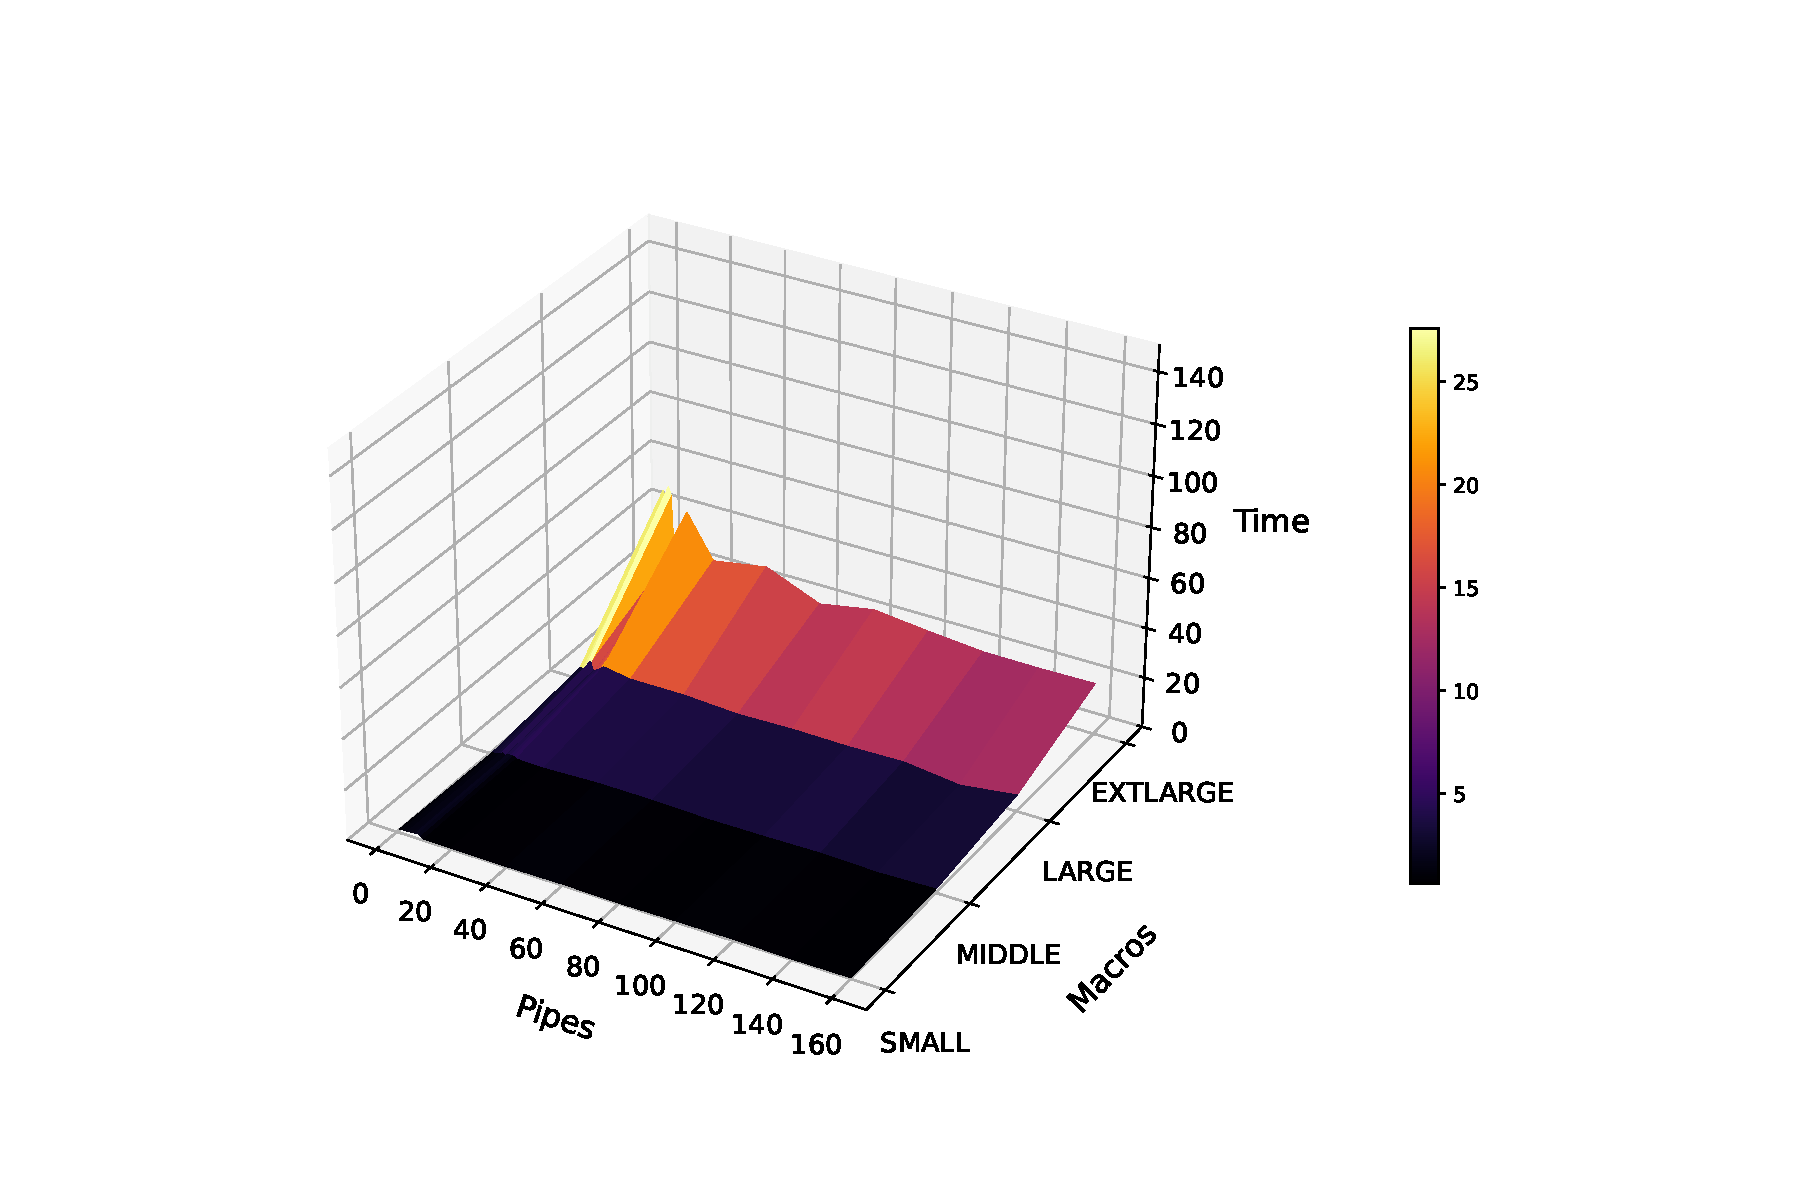
\includegraphics[width=0.8\textwidth]{../graph/task_o3.pdf} \\
    \small \it
    График 6.1
\end{center}

\begin{center}
    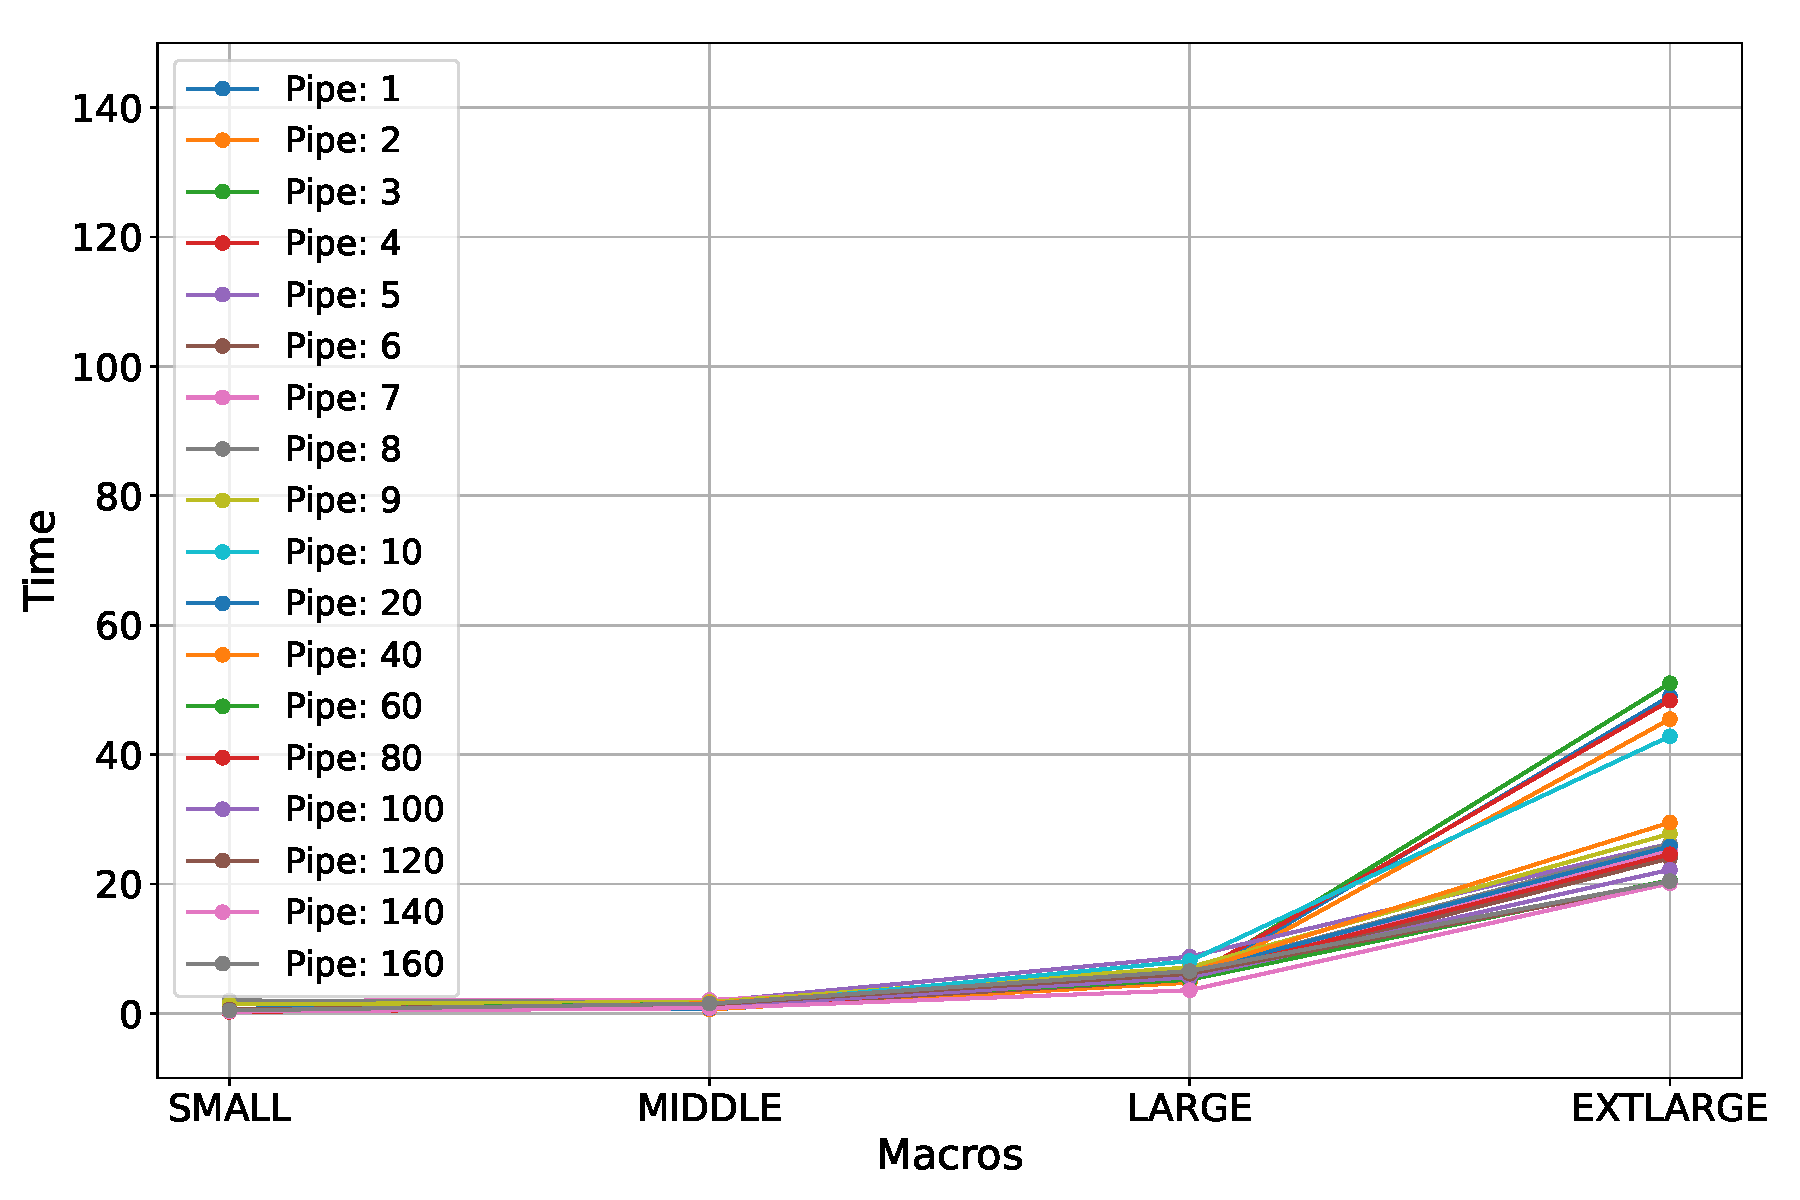
\includegraphics[width=0.6\textwidth]{../graph/task_o31.pdf} \\
    \small \it
    График 6.2\\ Графики 6.1, 6.2 --- Зависимость времени работы программы от объема входных данных и количества потоков при оптимизации с помощью директивы \texttt{task} и флага \texttt{-O3}.
\end{center}

\begin{center}
    \begin{tabular}{l | l l l l l l l l l}
        & \texttt{1} & \texttt{2} & \texttt{3} & \texttt{4} & \texttt{5} & \texttt{6} & \texttt{7} & \texttt{8} & \texttt{9} \\
        \hline
        \texttt{SMALL}    & $1.43$ & $1.56$ & $1.66$ & $1.49$ & $1.73$ & $1.7$ & $1.95$ & $2.0$ & $1.41$ \\
        \texttt{MIDDLE}   & $0.6$  & $0.62$ & $0.96$ & $1.08$ & $1.84$ & $0.92$ & $2.06$ & $1.74$ & $1.76$ \\
        \texttt{LARGE}    & $4.86$ & $4.75$ & $5.3$  & $5.61$ & $8.77$ & $5.2$ & $5.81$ & $6.38$ & $7.13$ \\
        \texttt{EXTLARGE} & $49.02$ & $45.48$ & $51.03$ & $48.35$ & $26.24$ & $23.97$ & $25.17$ & $26.19$ & $27.75$ \\
        \vspace{0.4cm}\\
        & \texttt{10} & \texttt{20} & \texttt{40} & \texttt{60} & \texttt{80} & \texttt{100} & \texttt{120} & \texttt{140} & \texttt{160} \\
        \hline
        \texttt{SMALL}    & $0.53$ & $0.47$ & $0.3$  & $0.55$ & $0.23$ & $0.52$ & $0.61$ & $0.28$ & $0.45$ \\
        \texttt{MIDDLE}   & $1.03$ & $0.74$ & $1.57$ & $1.5$  & $0.87$ & $1.03$ & $1.39$ & $0.81$ & $1.51$ \\
        \texttt{LARGE}    & $6.33$ & $6.41$ & $5.2$  & $5.8$  & $5.58$ & $6.13$ & $3.58$ & $6.55$ & $8.1$  \\
        \texttt{EXTLARGE} & $25.8$ & $29.49$ & $20.59$ & $24.59$ & $22.2$ & $20.24$ & $20.11$ & $20.45$ & $42.83$ \\
    \end{tabular}\\
    \vspace{0.3cm}
    \small \it
    Таблица 6. Результаты оптимизации с помощью директивы \texttt{task} и флага \texttt{-O3}. Значения указаны в секундах и округлены до сотых.
\end{center}
\newpage

\subsection*{Выводы об OpenMP}
\addcontentsline{toc}{subsection}{Выводы об OpenMP}
После реализации программ и проведения тестов можно сделать следующие выводы:

\begin{itemize}
    \item \textbf{Малые (\texttt{SMALL}) и средние (\texttt{MIDDLE}) наборы данных:} Для малых и средних наборов данных директива \texttt{task} показывает лучшую производительность. Например, для набора данных \texttt{MIDDLE} при одном потоке директива \texttt{task} работает быстрее, чем \texttt{for}. Это указывает на то, что \texttt{task} более эффективно распределяет задачи между потоками, особенно когда задачи относительно малы.
    \item \textbf{Большие (\texttt{LARGE}) и экстремально большие (\texttt{EXTLARGE}) наборы данных:} Для больших данных различия между \texttt{for} и \texttt{task} становятся менее выраженными. Для набора "\texttt{LARGE}" при большем числе потоков директива \texttt{for} работает быстрее, чем \texttt{task}. Это может свидетельствовать о том, что для больших данных дополнительная нагрузка на создание и синхронизацию задач в \texttt{task} становится более значимой.
\end{itemize}

Кроме того, выполнение программы не всегда ускоряется с увеличением числа потоков. Например, при использовании директивы \texttt{for}, для экстремально больших наборов данных оптимальное число потоков находится в диапазоне от 60 до 80. При увеличении числа потоков время выполнения перестает уменьшаться из-за накладных расходов на создание и синхронизацию дополнительных потоков. Особенно для небольших данных использование слишком большого числа потоков может замедлить выполнение программы, поскольку накладные расходы на создание потоков становятся значительными.


\subsubsection*{Влияние флагов компиляции}
\addcontentsline{toc}{subsubsection}{Влияние флагов компиляции}

\begin{itemize}
    \item \texttt{-O2}: Применение флага \texttt{-O2} значительно уменьшает время выполнения программы по сравнению с базовой версией. Это связано с улучшением работы с кэшированием данных и оптимизацией циклов.
    \item \texttt{-O3}: Флаг \texttt{-O3} ещё сильнее оптимизирует программу, что особенно заметно при использовании директивы \texttt{for} для большого числа потоков на больших наборах данных. Однако для некоторых случаев чрезмерная агрессивность оптимизаций может привести к ухудшению производительности из-за дополнительных вычислений, которые не всегда оправданы.
\end{itemize}
\newpage


\section*{MPI}
\addcontentsline{toc}{section}{MPI}

\subsection*{Параллелизация при помощи MPI}
\addcontentsline{toc}{subsection}{Параллелизация при помощи MPI}

\subsubsection*{Внесенные изменения}
\addcontentsline{toc}{subsubsection}{Внесенные изменения}
Для преобразования последовательной программы в параллельную с использованием MPI были внесены следующие изменения:

\begin{itemize}
    \item Добавлены вызовы инициализации и завершения работы библиотеки MPI: \texttt{MPI\_Init}, \texttt{MPI\_Finalize}, а также определение числа процессов посредством \texttt{MPI\_Comm\_size} и получение ранга каждого процесса с помощью \texttt{MPI\_Comm\_rank}.
    
    \item Массивы в программе распределены по измерению \texttt{i}, так что каждый процесс обрабатывает лишь подмассив, соответствующий определённому диапазону индексов по оси \texttt{i}. Для этого полный диапазон \texttt{i} (от \texttt{0} до \texttt{imax-1}) был разделён на примерно равные блоки по числу процессов, учитывая возможный остаток при неделимости длины массива на число процессов. Таким образом, если существует \texttt{size} процессов, то каждый процесс с рангом \texttt{rank} получает свой участок \texttt{[i\_start, i\_end]}, причём значения \texttt{i\_start} и \texttt{i\_end} вычисляются исходя из общего числа процессов и текущего ранга.
    
    \item Реализован обмен граничными слоями между соседями по оси \texttt{i} с помощью неблокирующих передач \texttt{MPI\_Isend} и \texttt{MPI\_Irecv}, что обеспечивает корректную обработку внутренних точек при вычислениях.
    
    \item Для сбора и агрегирования локальных результатов, таких как ошибка \texttt{gosa}, применена операция \texttt{MPI\_Allreduce}, позволяющая получить глобальное значение ошибки.
    
    \item Функция измерения времени \texttt{second()} заменена на \texttt{MPI\_Wtime()}, обеспечивающую синхронизированное измерение времени в параллельном режиме.
\end{itemize}
\newpage

\subsubsection*{Код программы}
\addcontentsline{toc}{subsubsection}{Код программы}
\begin{lstlisting}
#include <mpi.h>
#include <stdio.h>
#include <sys/time.h>

#define SMALL

#ifdef SMALL
#define MIMAX 65
#define MJMAX 33
#define MKMAX 33
#endif

#ifdef MIDDLE
#define MIMAX 129
#define MJMAX 65
#define MKMAX 65
#endif

#ifdef LARGE
#define MIMAX 257
#define MJMAX 129
#define MKMAX 129
#endif

#ifdef EXTLARGE
#define MIMAX 513
#define MJMAX 257
#define MKMAX 257
#endif

#define NN 200

float jacobi(int, int, int, int);
void initmt(int, int, int, int);

static float p[MIMAX][MJMAX][MKMAX];
static float a[MIMAX][MJMAX][MKMAX][4], b[MIMAX][MJMAX][MKMAX][3],
    c[MIMAX][MJMAX][MKMAX][3];
static float bnd[MIMAX][MJMAX][MKMAX];
static float wrk1[MIMAX][MJMAX][MKMAX], wrk2[MIMAX][MJMAX][MKMAX];

static int imax, jmax, kmax;
static float omega;

void initmt(int i_start, int i_end, int jmax, int kmax) {
    int i, j, k;
    for (i = i_start; i <= i_end; i++)
        for (j = 0; j < jmax; ++j)
            for (k = 0; k < kmax; ++k) {
                a[i][j][k][0] = 1.0;
                a[i][j][k][1] = 1.0;
                a[i][j][k][2] = 1.0;
                a[i][j][k][3] = 1.0 / 6.0;
                b[i][j][k][0] = 0.0;
                b[i][j][k][1] = 0.0;
                b[i][j][k][2] = 0.0;
                c[i][j][k][0] = 1.0;
                c[i][j][k][1] = 1.0;
                c[i][j][k][2] = 1.0;
                p[i][j][k] =
                    (float)(k * k) / (float)((kmax - 1) * (kmax - 1));
                wrk1[i][j][k] = 0.0;
                bnd[i][j][k] = 1.0;
                wrk2[i][j][k] = 0.0;
            }
}

float jacobi(int nn, int i_start, int i_end, int size) {
    int i, j, k, n;
    float gosa_local, gosa_global;
    int rank;
    MPI_Comm_rank(MPI_COMM_WORLD, &rank);

    int left = (rank == 0) ? MPI_PROC_NULL : rank - 1;
    int right = (rank == size - 1) ? MPI_PROC_NULL : rank + 1;

    static float send_left[MJMAX][MKMAX], send_right[MJMAX][MKMAX];
    static float recv_left[MJMAX][MKMAX], recv_right[MJMAX][MKMAX];

    for (n = 0; n < nn; ++n) {
        if (i_start > 0) {
            for (j = 0; j < jmax; j++)
                for (k = 0; k < kmax; k++)
                    send_left[j][k] = p[i_start][j][k];
        }
        if (i_end < imax - 1) {
            for (j = 0; j < jmax; j++)
                for (k = 0; k < kmax; k++)
                    send_right[j][k] = p[i_end][j][k];
        }

        MPI_Request reqs[4];
        int req_count = 0;

        if (left != MPI_PROC_NULL) {
            MPI_Isend(&send_left[0][0], jmax * kmax, MPI_FLOAT, left, 0,
                      MPI_COMM_WORLD, &reqs[req_count++]);
            MPI_Irecv(&recv_left[0][0], jmax * kmax, MPI_FLOAT, left, 1,
                      MPI_COMM_WORLD, &reqs[req_count++]);
        }
        if (right != MPI_PROC_NULL) {
            MPI_Isend(&send_right[0][0], jmax * kmax, MPI_FLOAT, right, 1,
                      MPI_COMM_WORLD, &reqs[req_count++]);
            MPI_Irecv(&recv_right[0][0], jmax * kmax, MPI_FLOAT, right, 0,
                      MPI_COMM_WORLD, &reqs[req_count++]);
        }

        MPI_Waitall(req_count, reqs, MPI_STATUSES_IGNORE);

        if (left != MPI_PROC_NULL) {
            for (j = 0; j < jmax; j++)
                for (k = 0; k < kmax; k++)
                    p[i_start - 1][j][k] = recv_left[j][k];
        }
        if (right != MPI_PROC_NULL) {
            for (j = 0; j < jmax; j++)
                for (k = 0; k < kmax; k++)
                    p[i_end + 1][j][k] = recv_right[j][k];
        }

        gosa_local = 0.0f;

        for (i = (i_start > 1 ? i_start : 1);
             i <= (i_end < imax - 2 ? i_end : imax - 2); i++)
            for (j = 1; j < jmax - 1; ++j)
                for (k = 1; k < kmax - 1; ++k) {
                    float s0 = a[i][j][k][0] * p[i + 1][j][k] +
                               a[i][j][k][1] * p[i][j + 1][k] +
                               a[i][j][k][2] * p[i][j][k + 1] +
                               b[i][j][k][0] *
                                   (p[i + 1][j + 1][k] - p[i + 1][j - 1][k] -
                                    p[i - 1][j + 1][k] + p[i - 1][j - 1][k]) +
                               b[i][j][k][1] *
                                   (p[i][j + 1][k + 1] - p[i][j - 1][k + 1] -
                                    p[i][j + 1][k - 1] + p[i][j - 1][k - 1]) +
                               b[i][j][k][2] *
                                   (p[i + 1][j][k + 1] - p[i - 1][j][k + 1] -
                                    p[i + 1][j][k - 1] + p[i - 1][j][k - 1]) +
                               c[i][j][k][0] * p[i - 1][j][k] +
                               c[i][j][k][1] * p[i][j - 1][k] +
                               c[i][j][k][2] * p[i][j][k - 1] + wrk1[i][j][k];

                    float ss =
                        (s0 * a[i][j][k][3] - p[i][j][k]) * bnd[i][j][k];
                    gosa_local += ss * ss;
                    wrk2[i][j][k] = p[i][j][k] + omega * ss;
                }

        for (i = (i_start > 1 ? i_start : 1);
             i <= (i_end < imax - 2 ? i_end : imax - 2); i++)
            for (j = 1; j < jmax - 1; ++j)
                for (k = 1; k < kmax - 1; ++k)
                    p[i][j][k] = wrk2[i][j][k];

        MPI_Allreduce(&gosa_local, &gosa_global, 1, MPI_FLOAT, MPI_SUM,
                      MPI_COMM_WORLD);
    }

    return gosa_global;
}

int main(int argc, char* argv[]) {
    int i, j, k;
    int rank, size;
    double cpu0, cpu1, nflop, xmflops2, score;
    float gosa_local, gosa;

    MPI_Init(&argc, &argv);
    MPI_Comm_size(MPI_COMM_WORLD, &size);
    MPI_Comm_rank(MPI_COMM_WORLD, &rank);

    omega = 0.8;
    imax = MIMAX - 1;
    jmax = MJMAX - 1;
    kmax = MKMAX - 1;

    int i_block = imax / size;
    int rest = imax % size;
    int i_start, i_end;
    if (rank < rest) {
        i_block = imax / size + 1;
        i_start = rank * i_block;
        i_end = i_start + i_block - 1;
    } else {
        i_block = imax / size;
        i_start = rest * ((imax / size) + 1) + (rank - rest) * i_block;
        i_end = i_start + i_block - 1;
    }

    initmt(i_start, i_end, jmax, kmax);

    if (rank == 0) {
        printf("mimax = %d mjmax = %d mkmax = %d\n", MIMAX, MJMAX, MKMAX);
        printf("imax = %d jmax = %d kmax = %d\n", imax, jmax, kmax);
    }

    MPI_Barrier(MPI_COMM_WORLD);
    cpu0 = MPI_Wtime();

    gosa = jacobi(NN, i_start, i_end, size);

    MPI_Barrier(MPI_COMM_WORLD);
    cpu1 = MPI_Wtime();

    nflop = (kmax - 2) * (jmax - 2) * (imax - 2) * 34;

    if (rank == 0) {
        if (cpu1 != 0.0)
            xmflops2 = nflop / cpu1 * 1.0e-6 * (float)NN;
        else
            xmflops2 = 0.0;

        score = xmflops2 / 32.27;

        printf("%f,\n", cpu1 - cpu0);
        printf("cpu : %f sec.\n", cpu1 - cpu0);
        printf("Loop executed for %d times\n", NN);
        printf("Gosa : %e \n", gosa);
        printf("MFLOPS measured : %f\n", xmflops2);
        printf("Score based on MMX Pentium 200MHz : %f\n", score);
    }

    MPI_Finalize();
    return (0);
}
\end{lstlisting}
\newpage


\subsubsection*{Тестирование программы на Polus}
\addcontentsline{toc}{subsubsection}{Тестирование программы на Polus}
\begin{center}
    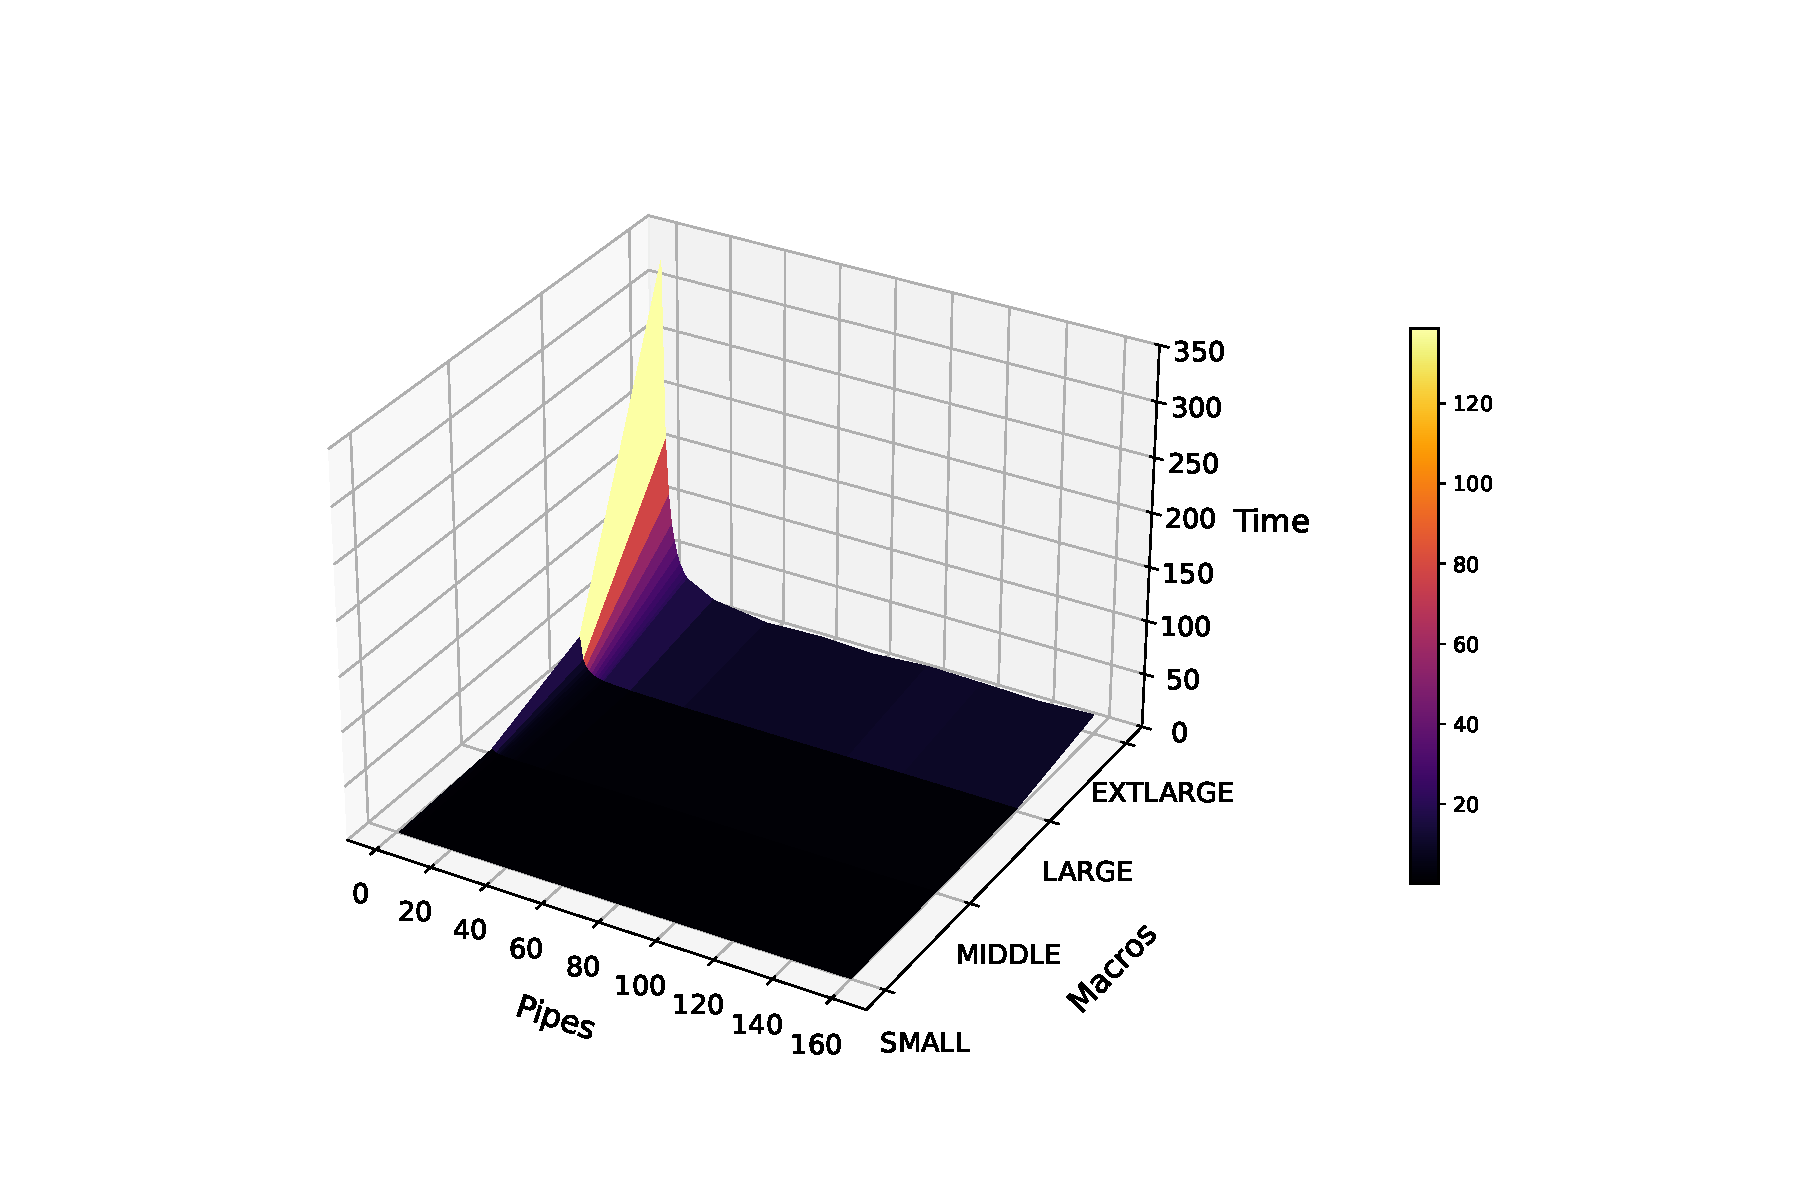
\includegraphics[width=0.8\textwidth]{../graph/mpi.pdf} \\
    \small \it
    График 7.1
\end{center}

\begin{center}
    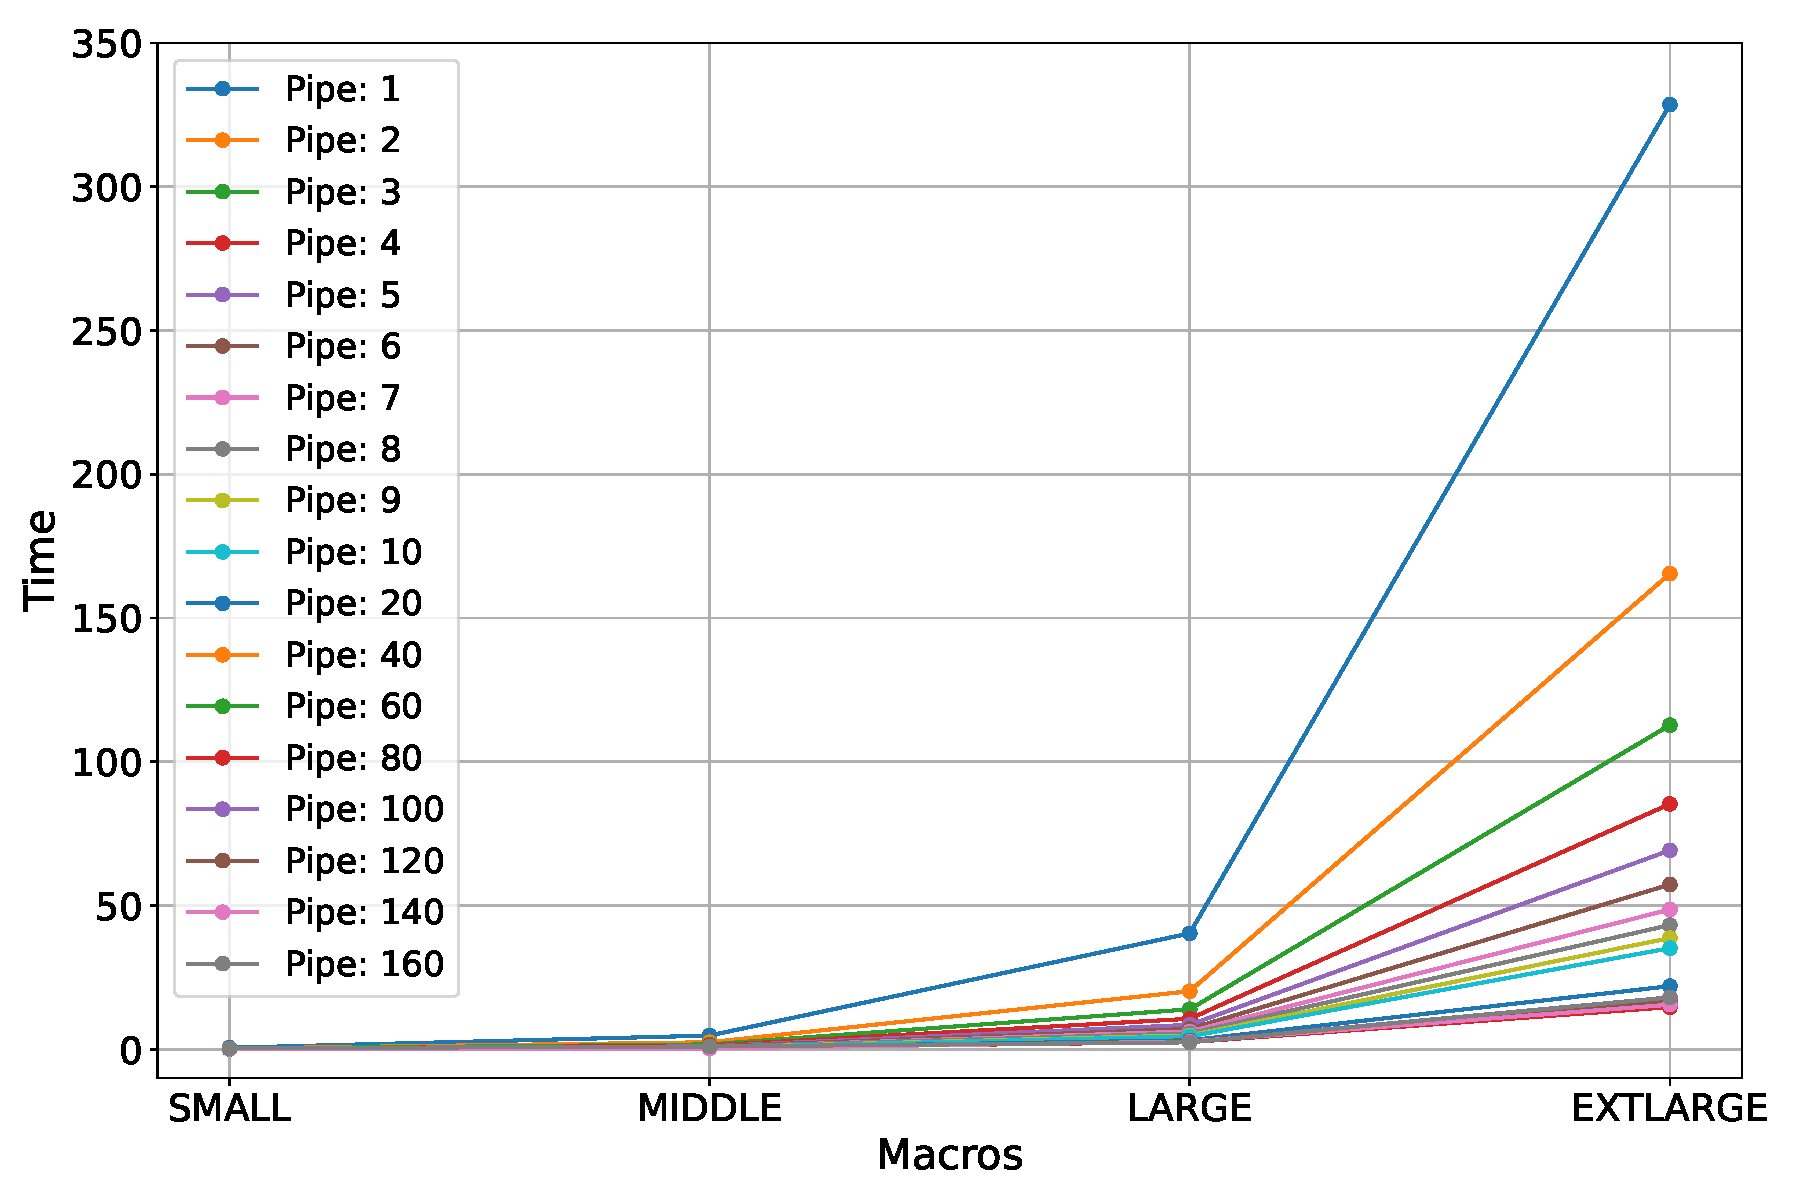
\includegraphics[width=0.6\textwidth]{../graph/mpi1.pdf} \\
    \small \it
    График 7.2\\ Графики 7.1, 7.2 --- Зависимость времени работы программы от объема входных данных и количества потоков с помощью \texttt{mpi}.
\end{center}

\begin{center}
    \begin{tabular}{l | l l l l l l l l l}
        & \texttt{1} & \texttt{2} & \texttt{3} & \texttt{4} & \texttt{5} & \texttt{6} & \texttt{7} & \texttt{8} & \texttt{9} \\
        \hline
        \texttt{SMALL}    & $0.54$ & $0.28$ & $0.24$ & $0.16$ & $0.12$ & $0.22$ & $0.11$ & $0.11$ & $0.15$ \\
        \texttt{MIDDLE}   & $4.78$ & $2.47$ & $1.71$ & $1.31$ & $1.05$ & $0.98$ & $0.77$ & $0.89$ & $0.66$ \\
        \texttt{LARGE}    & $40.32$ & $20.21$ & $13.93$ & $10.62$ & $8.51$ & $7.10$ & $6.20$ & $5.54$ & $4.85$ \\
        \texttt{EXTLARGE} & $328.54$ & $165.42$ & $112.75$ & $85.33$ & $69.20$ & $57.30$ & $48.63$ & $43.20$ & $38.70$ \\
        \vspace{0.4cm}\\
        & \texttt{10} & \texttt{20} & \texttt{40} & \texttt{60} & \texttt{80} & \texttt{100} & \texttt{120} & \texttt{140} & \texttt{160} \\
        \hline
        \texttt{SMALL}    & $0.15$ & $0.11$ & $0.10$ & $0.06$ & $0.06$ & $0.07$ & $0.07$ & $0.19$ & $0.36$ \\
        \texttt{MIDDLE}   & $0.66$ & $0.54$ & $0.51$ & $0.55$ & $0.53$ & $0.49$ & $0.53$ & $0.31$ & $0.98$ \\
        \texttt{LARGE}    & $4.51$ & $3.14$ & $2.54$ & $2.60$ & $2.49$ & $2.57$ & $2.80$ & $2.70$ & $2.43$ \\
        \texttt{EXTLARGE} & $35.19$ & $21.96$ & $14.78$ & $16.61$ & $14.68$ & $18.08$ & $17.06$ & $15.52$ & $18.06$ \\
    \end{tabular}\\
    \vspace{0.3cm}
    \small \it
    Таблица 7.  Результаты оптимизации с помощью \texttt{mpi}. Значения указаны в секундах и округлены до сотых.
\end{center}
\newpage

\subsubsection*{Тестирование программы на Polus. Флаг оптимизации \texttt{-O2}}
\addcontentsline{toc}{subsubsection}{Тестирование программы на Polus. Флаг оптимизации \texttt{-O2}}
\begin{center}
    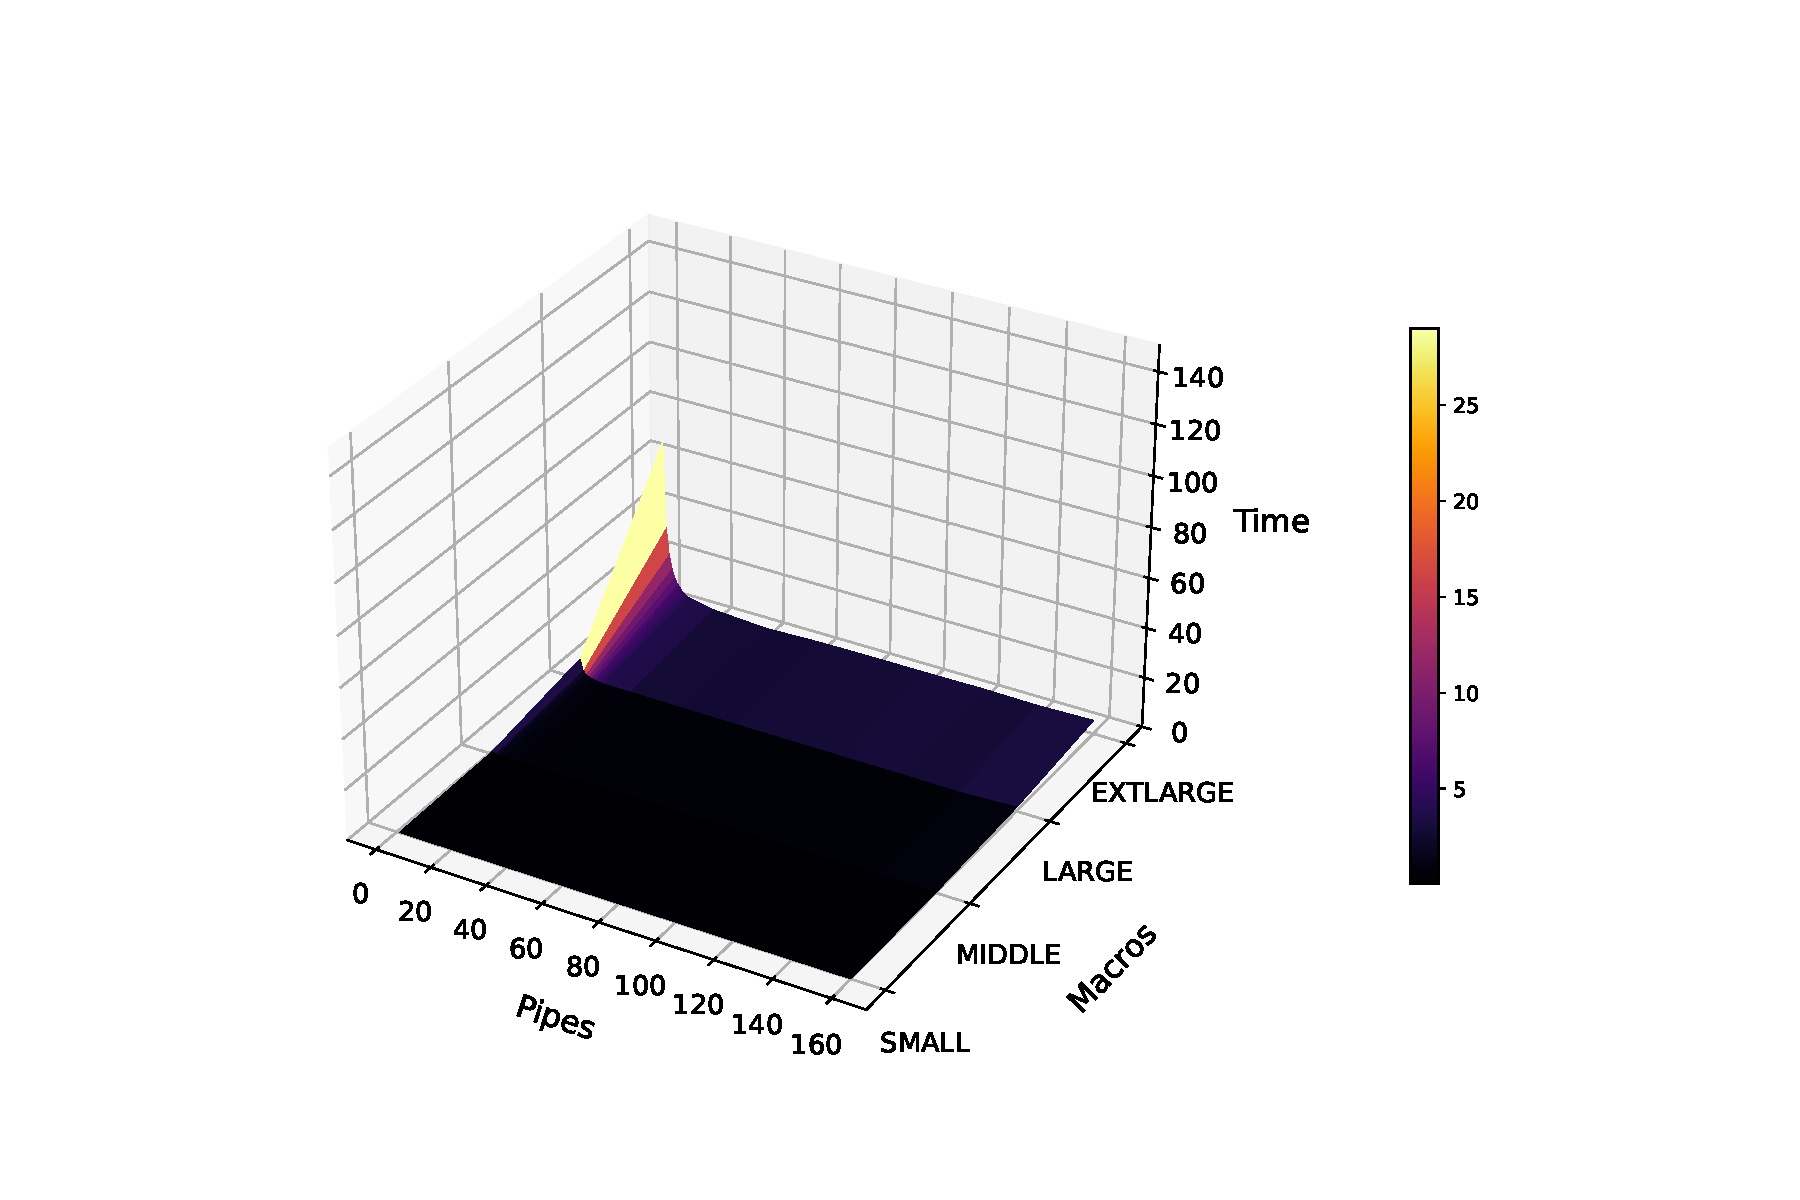
\includegraphics[width=0.8\textwidth]{../graph/mpi_o2.pdf} \\
    \small \it
    График 8.1
\end{center}

\begin{center}
    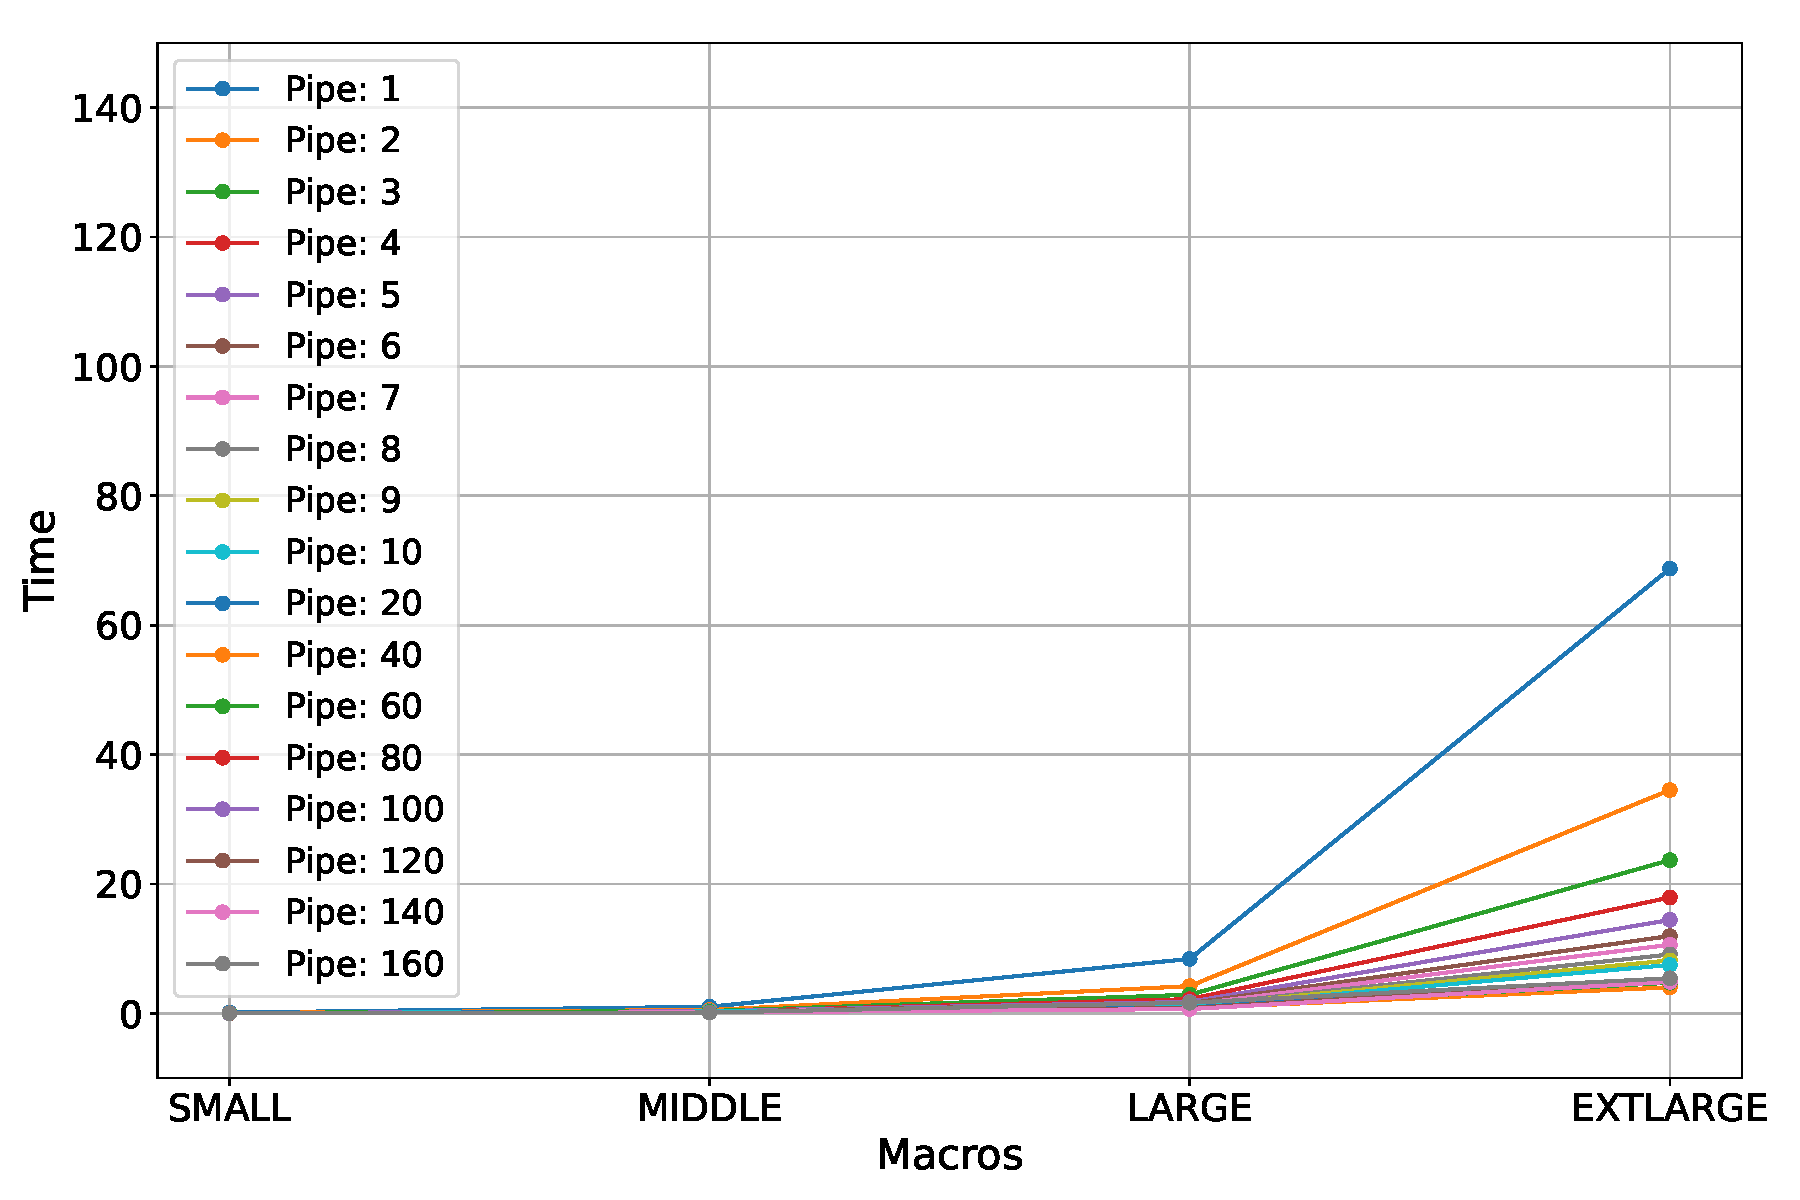
\includegraphics[width=0.6\textwidth]{../graph/mpi_o21.pdf} \\
    \small \it
    График 8.2\\ Графики 8.1, 8.2  --- Зависимость времени работы программы от объема входных данных и количества потоков с помощью \texttt{mpi} и флага \texttt{-O2}.
\end{center}

\begin{center}
    \begin{tabular}{l | l l l l l l l l l}
        & \texttt{1} & \texttt{2} & \texttt{3} & \texttt{4} & \texttt{5} & \texttt{6} & \texttt{7} & \texttt{8} & \texttt{9} \\
        \hline
        \texttt{SMALL}    & $0.12$ & $0.06$ & $0.07$ & $0.05$ & $0.04$ & $0.06$ & $0.03$ & $0.04$ & $0.04$ \\
        \texttt{MIDDLE}   & $1.02$ & $0.52$ & $0.36$ & $0.29$ & $0.33$ & $0.25$ & $0.23$ & $0.23$ & $0.19$ \\
        \texttt{LARGE}    & $8.42$ & $4.21$ & $2.88$ & $2.20$ & $1.78$ & $1.57$ & $1.35$ & $1.18$ & $1.14$ \\
        \texttt{EXTLARGE} & $68.74$ & $34.52$ & $23.69$ & $17.92$ & $14.45$ & $11.95$ & $10.61$ & $9.11$ & $8.19$ \\
        \vspace{0.4cm}\\
        & \texttt{10} & \texttt{20} & \texttt{40} & \texttt{60} & \texttt{80} & \texttt{100} & \texttt{120} & \texttt{140} & \texttt{160} \\
        \hline
        \texttt{SMALL}    & $0.04$ & $0.05$ & $0.03$ & $0.03$ & $0.02$ & $0.02$ & $0.03$ & $0.03$ & $0.03$ \\
        \texttt{MIDDLE}   & $0.29$ & $0.21$ & $0.20$ & $0.21$ & $0.14$ & $0.15$ & $0.15$ & $0.15$ & $0.13$ \\
        \texttt{LARGE}    & $0.99$ & $0.90$ & $0.80$ & $0.81$ & $0.76$ & $0.75$ & $0.82$ & $0.67$ & $1.65$ \\
        \texttt{EXTLARGE} & $7.49$ & $5.35$ & $4.02$ & $4.74$ & $4.93$ & $4.98$ & $5.16$ & $4.87$ & $5.43$ \\
    \end{tabular}\\
    \vspace{0.3cm}
    \small \it
    Таблица 8.  Результаты оптимизации с помощью \texttt{mpi} и флага \texttt{-O2}. Значения указаны в секундах и округлены до сотых.
\end{center}
\newpage

\subsubsection*{Тестирование программы на Polus. Флаг оптимизации \texttt{-O3}}
\addcontentsline{toc}{subsubsection}{Тестирование программы на Polus. Флаг оптимизации \texttt{-O3}}
\begin{center}
    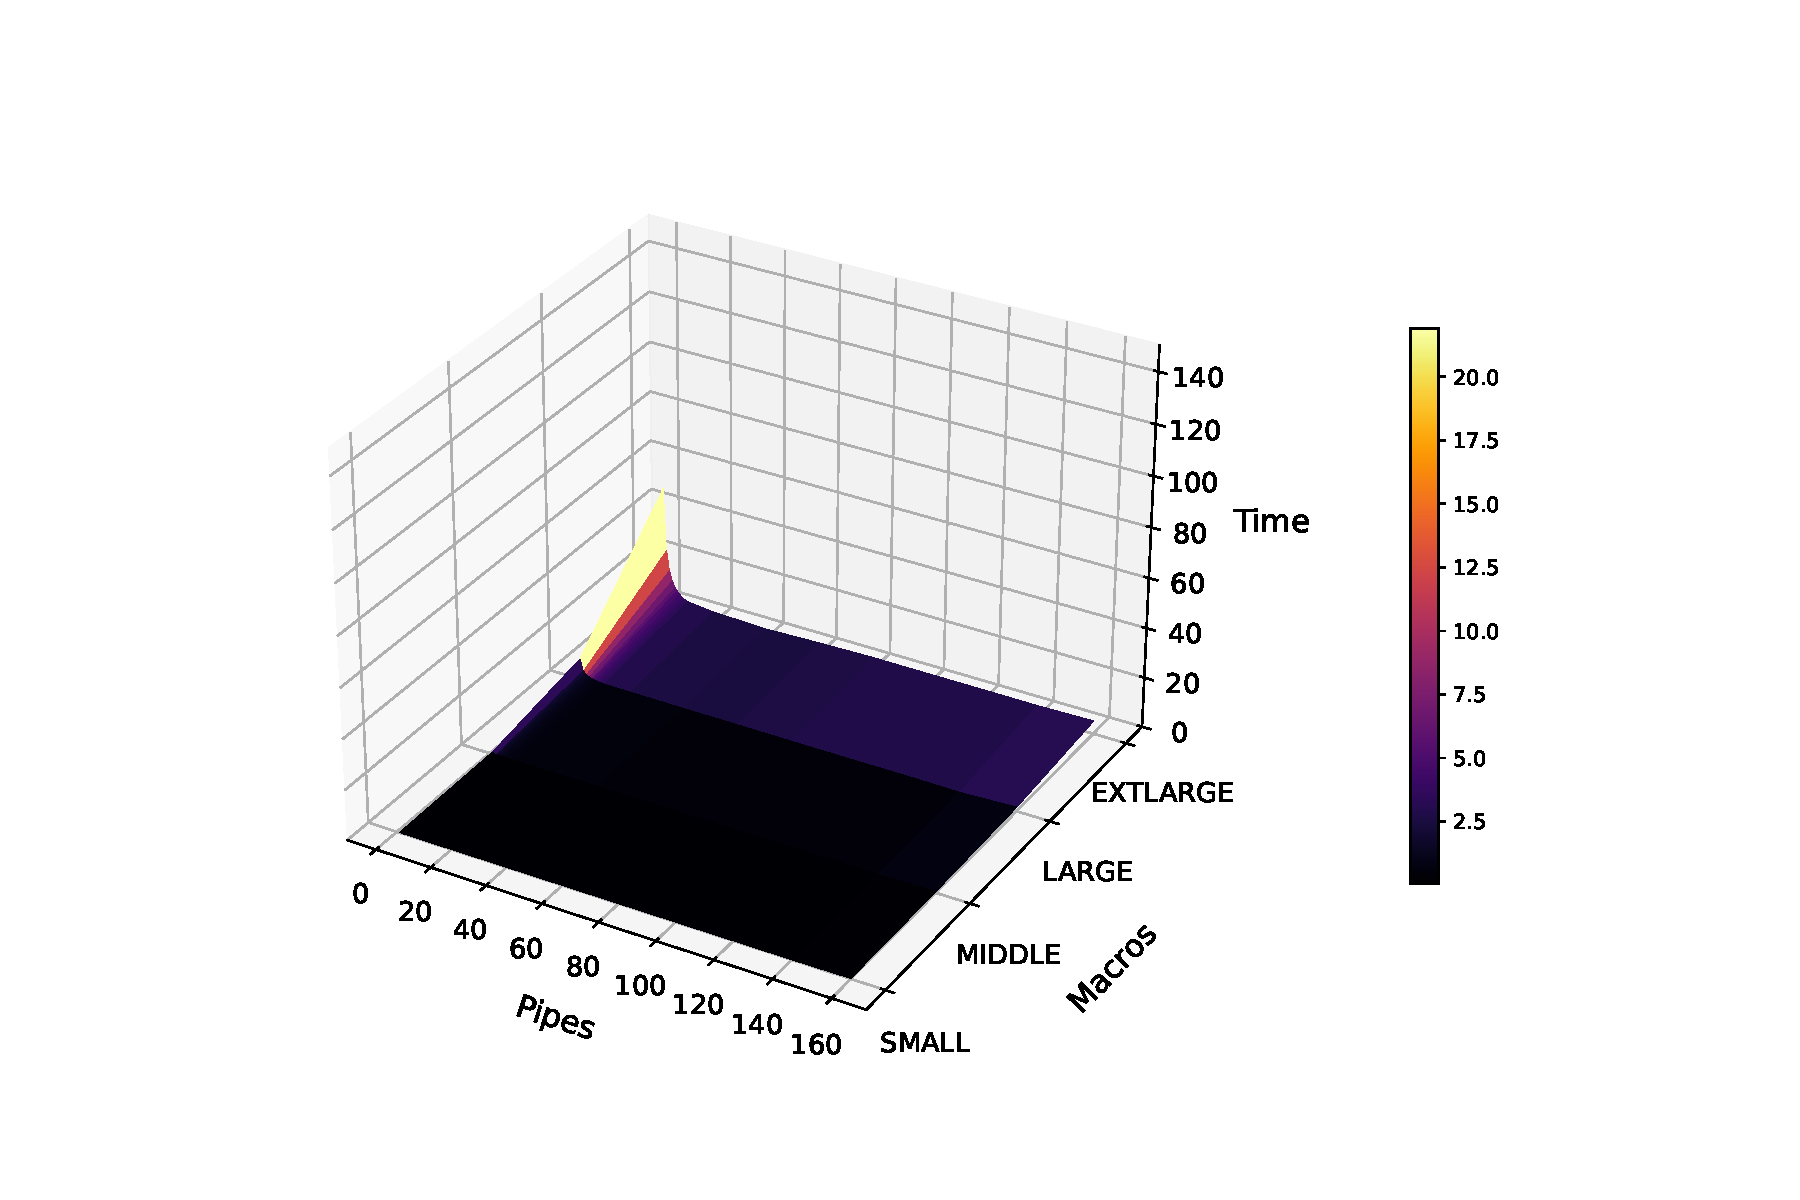
\includegraphics[width=0.8\textwidth]{../graph/mpi_o3.pdf} \\
    \small \it
    График 9.1
\end{center}

\begin{center}
    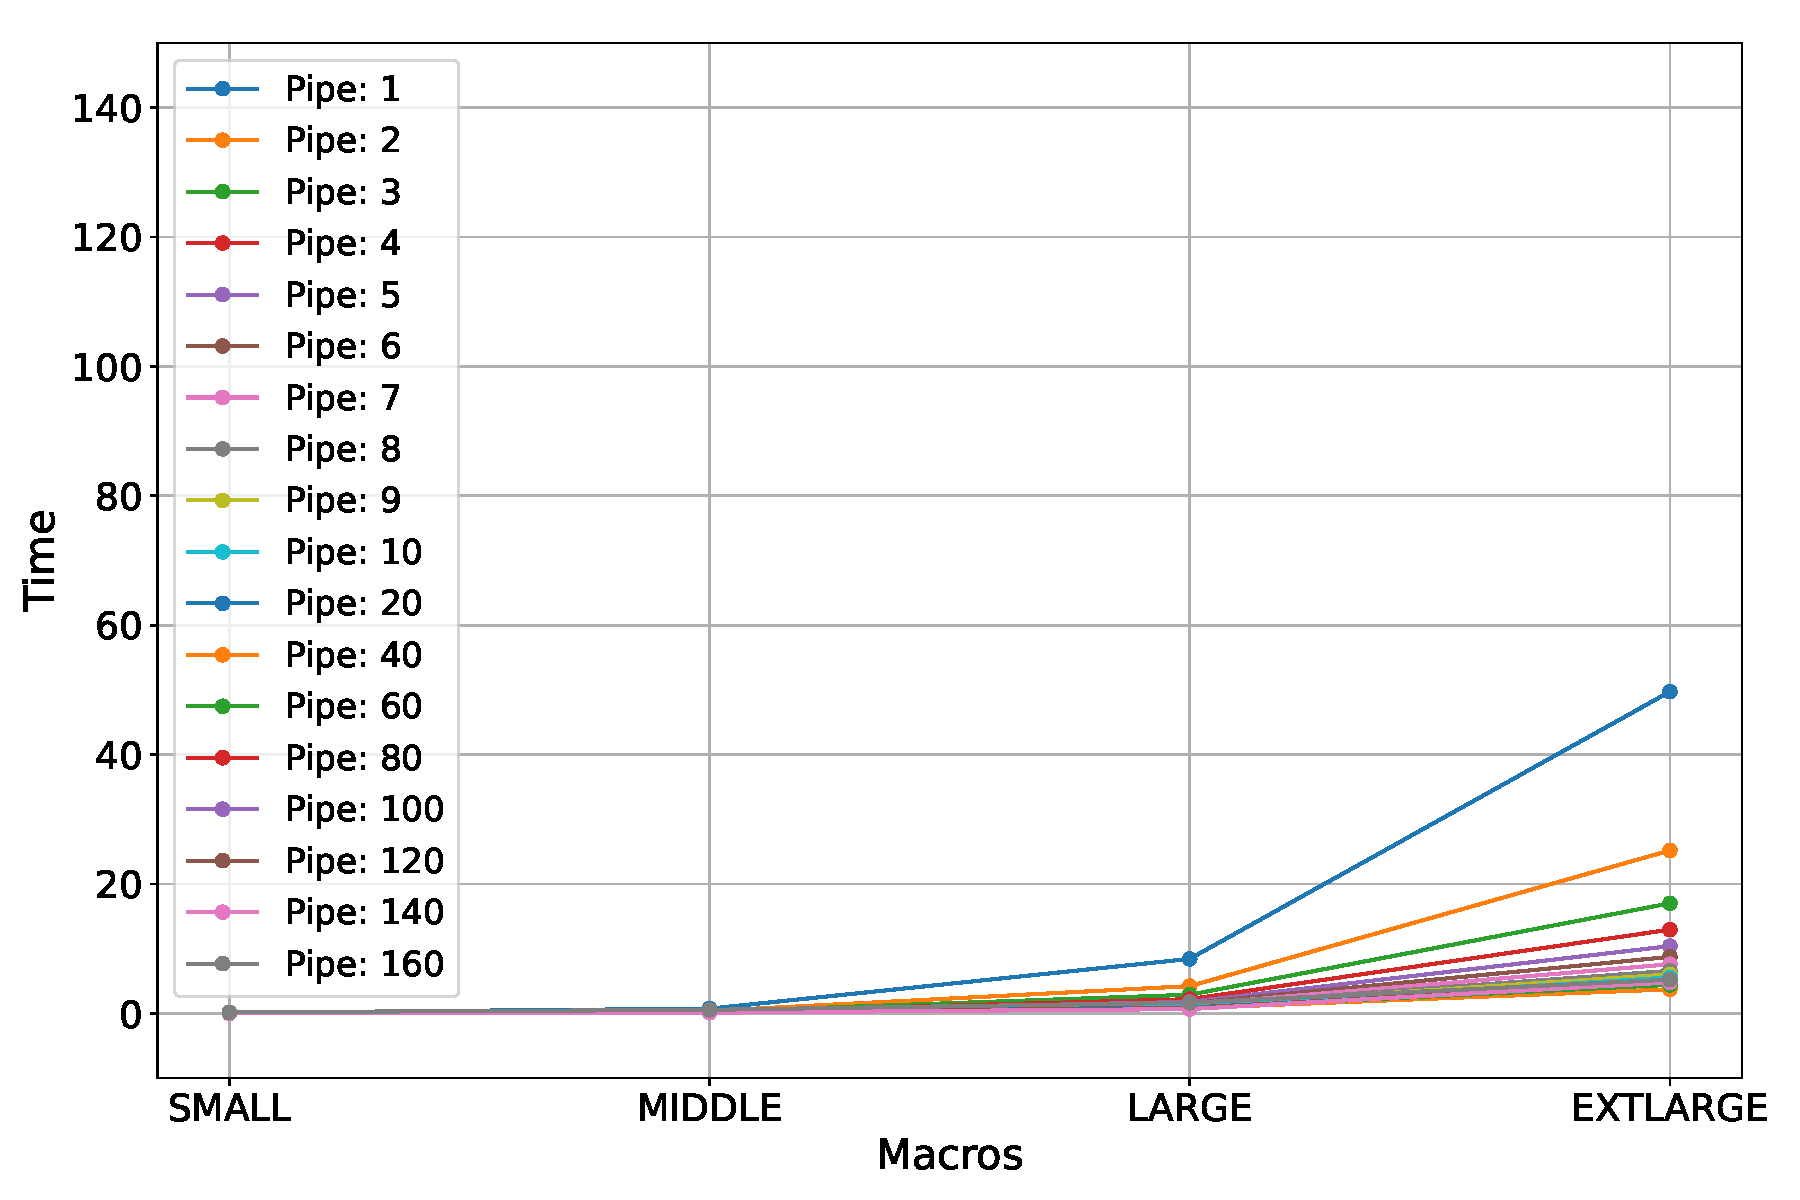
\includegraphics[width=0.6\textwidth]{../graph/mpi_o31.pdf} \\
    \small \it
    График 9.2\\ Графики 9.1, 9.2 --- Зависимость времени работы программы от объема входных данных и количества потоков с помощью \texttt{mpi} и флага \texttt{-O3}.
\end{center}

\begin{center}
    \begin{tabular}{l | l l l l l l l l l}
        & \texttt{1} & \texttt{2} & \texttt{3} & \texttt{4} & \texttt{5} & \texttt{6} & \texttt{7} & \texttt{8} & \texttt{9} \\
        \hline
        \texttt{SMALL}    & $0.08$ & $0.04$ & $0.03$ & $0.04$ & $0.03$ & $0.04$ & $0.02$ & $0.04$ & $0.03$ \\
        \texttt{MIDDLE}   & $0.73$ & $0.37$ & $0.26$ & $0.21$ & $0.24$ & $0.18$ & $0.17$ & $0.15$ & $0.27$ \\
        \texttt{LARGE}    & $8.42$ & $4.21$ & $2.88$ & $2.20$ & $1.78$ & $1.57$ & $1.35$ & $1.18$ & $1.14$ \\
        \texttt{EXTLARGE} & $49.72$ & $25.18$ & $17.01$ & $12.94$ & $10.40$ & $8.74$ & $7.60$ & $6.57$ & $6.01$ \\
        \vspace{0.4cm}\\
        & \texttt{10} & \texttt{20} & \texttt{40} & \texttt{60} & \texttt{80} & \texttt{100} & \texttt{120} & \texttt{140} & \texttt{160} \\
        \hline
        \texttt{SMALL}    & $0.01$ & $0.04$ & $0.03$ & $0.03$ & $0.02$ & $0.02$ & $0.02$ & $0.02$ & $0.17$ \\
        \texttt{MIDDLE}   & $0.18$ & $0.22$ & $0.19$ & $0.16$ & $0.12$ & $0.13$ & $0.17$ & $0.11$ & $0.55$ \\
        \texttt{LARGE}    & $0.99$ & $0.90$ & $0.80$ & $0.81$ & $0.76$ & $0.75$ & $0.82$ & $0.67$ & $1.65$ \\
        \texttt{EXTLARGE} & $5.55$ & $4.42$ & $3.72$ & $4.42$ & $4.85$ & $4.82$ & $4.84$ & $4.79$ & $5.22$ \\
    \end{tabular}\\
    \vspace{0.3cm}
    \small \it
    Таблица 9. Результаты оптимизации с помощью \texttt{mpi} и флага \texttt{-O3}. Значения указаны в секундах и округлены до сотых.
\end{center}
\newpage

\subsection*{Выводы о MPI}
\addcontentsline{toc}{subsection}{Выводы о MPI}
После проведения анализа результатов тестирования программы с использованием MPI можно сделать следующие выводы:

\begin{itemize}
    \item \textbf{Малые (\texttt{SMALL}) наборы данных:} 
    Для малых наборов данных увеличение числа потоков не всегда приводит к улучшению производительности. Например, в базовой версии (\texttt{без флагов}) время выполнения существенно колеблется при большем количестве потоков. С применением флагов \texttt{-O2} и \texttt{-O3} ситуация становится стабильнее, но наибольшее ускорение наблюдается только при ограниченном числе потоков (до 20). Накладные расходы на синхронизацию потоков приводят к деградации производительности при большем числе потоков.

    \item \textbf{Средние (\texttt{MIDDLE}) наборы данных:} 
    Для средних наборов данных наблюдается значительное уменьшение времени выполнения с увеличением числа потоков, особенно при использовании флагов компиляции. Флаг \texttt{-O3} показывает наилучшую производительность для числа потоков от 10 до 80. Однако при увеличении потоков более 120 начинает проявляться эффект насыщения, и производительность стабилизируется либо ухудшается из-за накладных расходов.

    \item \textbf{Большие (\texttt{LARGE}) наборы данных:}
    Для больших данных оптимизация более заметна. Базовая версия программы демонстрирует монотонное улучшение производительности с увеличением числа потоков. Применение флагов \texttt{-O2} и \texttt{-O3} позволяет достичь значительно лучшего ускорения, особенно при числе потоков до 40. При этом флаг \texttt{-O3} показывает лучшее время выполнения, но производительность стабилизируется при большом числе потоков (от 80 и выше).

    \item \textbf{Экстремально большие (\texttt{EXTLARGE}) наборы данных:} 
    Для экстремально больших данных наибольшее ускорение достигается при использовании флагов \texttt{-O2} и \texttt{-O3}. Особенно заметен эффект флага \texttt{-O3}, который обеспечивает лучшее распределение нагрузки между потоками. Однако при большом числе потоков (свыше 100) производительность стабилизируется, а в некоторых случаях даже деградирует из-за накладных расходов на синхронизацию.
\end{itemize}

\subsubsection*{Влияние флагов компиляции}
\addcontentsline{toc}{subsubsection}{Влияние флагов компиляции}

\begin{itemize}
    \item \texttt{-O2}: Флаг \texttt{-O2} значительно улучшает производительность для всех наборов данных. Наибольший эффект наблюдается для средних (\texttt{MIDDLE}) и больших (\texttt{LARGE}) данных, где время выполнения сокращается более чем в два раза. Для экстремально больших (\texttt{EXTLARGE}) данных флаг обеспечивает стабильность при числе потоков от 80, снижая влияние синхронизации.

    \item \texttt{-O3}: Флаг \texttt{-O3} показывает лучшие результаты, особенно на больших (\texttt{LARGE}) и экстремально больших (\texttt{EXTLARGE}) данных, с максимальным ускорением при 60–80 потоках. Однако на малых (\texttt{SMALL}) данных или при числе потоков выше 140 агрессивные оптимизации иногда приводят к нестабильности из-за накладных расходов.
\end{itemize}
\newpage

\section*{Выводы}
\addcontentsline{toc}{section}{Выводы}
На основе результатов тестирования можно сделать следующие выводы о производительности реализаций параллелизма с использованием OpenMP (\texttt{for} и \texttt{task}) и MPI:

\begin{enumerate}
    \item \textbf{OpenMP (директива \texttt{for}):}
    \begin{itemize}
        \item Хорошо работает с относительно мелкими объемами данных (\texttt{SMALL} и \texttt{MIDDLE}).
        \item Демонстрирует стабильную производительность при увеличении числа потоков.
        \item При больших объемах данных (\texttt{LARGE} и \texttt{EXTLARGE}) производительность начинает снижаться, особенно если число потоков превышает оптимальное значение.
        \item Для больших данных использование оптимизаций (\texttt{-O2}, \texttt{-O3}) значительно улучшает производительность.
    \end{itemize}

    \item \textbf{OpenMP (директива \texttt{task}):}
    \begin{itemize}
        \item Эффективна на большом числе потоков при условии оптимизации. Однако в некоторых случаях наблюдается рост времени выполнения из-за накладных расходов на управление задачами.
        \item Показывает преимущество при обработке крупных данных (\texttt{LARGE} и \texttt{EXTLARGE}), особенно с оптимизациями компилятора.
        \item Меньше подходит для мелких объемов данных, где накладные расходы на управление задачами оказываются значительными.
    \end{itemize}

    \item \textbf{MPI:}
    \begin{itemize}
        \item Наиболее эффективна для очень больших объемов данных (\texttt{EXTLARGE}).
        \item Масштабируемость выше, чем у OpenMP, при условии правильного разбиения данных.
    \end{itemize}
\end{enumerate}
\newpage

\section*{Приложения}
\addcontentsline{toc}{section}{Приложения}
\begin{itemize}
    \item Прилагаемые файлы OpenMP:
    \begin{enumerate}
        \item Файл \texttt{for.c} --- реазация параллелизма при помощи директивы \texttt{for}. 
        \item Файл \texttt{task.c} --- реазация параллелизма при помощи директивы \texttt{task}. 
    \end{enumerate}
\end{itemize}

\begin{itemize}
    \item Прилагаемые файлы MPI:
    \begin{enumerate}
        \item Файл \texttt{mpi.c} --- реазация параллелизма при помощи \texttt{MPI}. 
    \end{enumerate}
\end{itemize}



\end{document}
